\documentclass[10pt]{article}
\usepackage{fullpage, graphicx, url}
\usepackage{hyperref}
\usepackage{placeins}
\setlength{\parskip}{1ex}
\setlength{\parindent}{0ex}
\title{User Manual}
\date{Version}
\author{}

\usepackage{wrapfig}


\begin{document}
\begin{titlepage}

\begin{center}
\vspace{3 cm}
\Huge \textbf{3Depict}\\[1.0cm]

\textsc{\Large Valued point cloud visualisation and analysis}\\
\hrulefill \\[1.0cm]

\begin{center}
 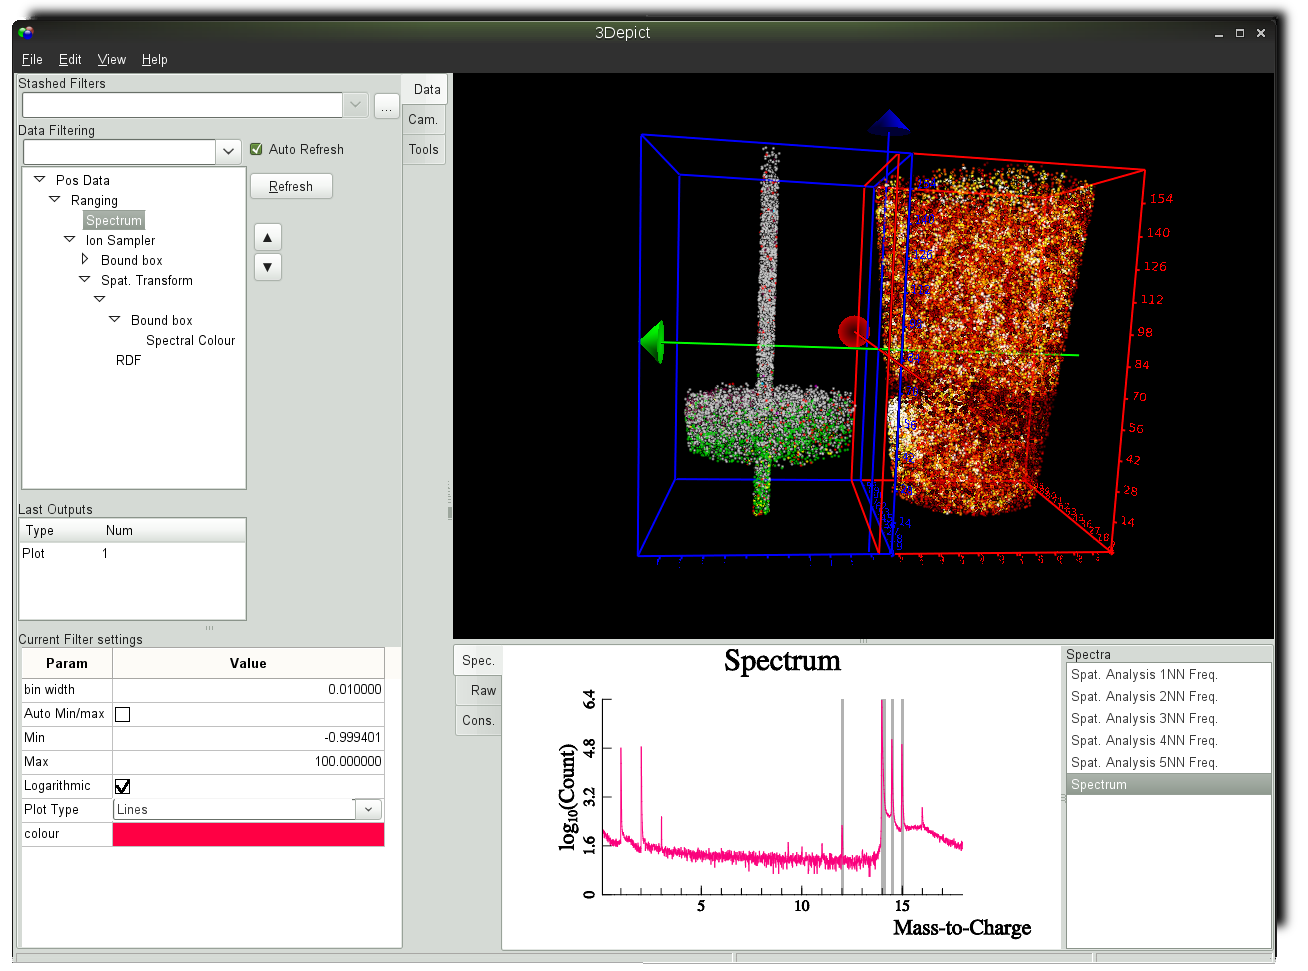
\includegraphics[width=\textwidth,keepaspectratio=true]{./figures/CoverImage.png}
 % CoverImage.png: 1308x957 pixel, 72dpi, 46.14x33.76 cm, bb=0 0 1308 957
\end{center}
\vspace{1.0 cm}


{ \Huge \bfseries User manual}\\[0.4cm]
\vspace{1.0 cm}


\begin{minipage}{0.5\textwidth}
\begin{flushleft} \large
\emph{Website:}\\
\url{http://threedepict.sourceforge.net/}\end{flushleft}
\end{minipage}
\begin{minipage}{0.3\textwidth}
\begin{flushright} \large
\emph{Version:} \\
 0.0.12, Nov 2012\end{flushright}
\end{minipage}

\vfill

\end{center}

\end{titlepage}
\clearpage
\pagenumbering{roman}
\tableofcontents
\clearpage
\pagenumbering{arabic}
\title{3Depict -- Valued point cloud visualisation and analysis}

\widowpenalty = 10000



\section{Foreword}
\subsection{Introduction}

\emph{3Depict} is an open source computer program designed for the analysis of point clouds with an associated scalar value. The program is designed around interactive data analysis, with a view to combine rapid feedback, ease of use and flexibility in a single system.  At time of writing, \emph{3Depict} is in the so-called ``alpha'' prototyping stage, and should be used where helpful, but may contain rough-edges.

\emph{3Depict} is designed purely for post-processing of 3D point data, and was originally primarily targeted to users of Atom Probe Tomography. Other users (\emph{e.g.} in astronomical, geospatial or digital preservation fields) may find the program useful, and are encouraged to seek assistance. 
 
\subsubsection{Background}

\emph{3Depict} attempts to fill a perceived need for freely available flexible point data visualisation. This program is designed to manipulate and modify point data in a way which the author has otherwise not found a suitable program to do.  
 
With this program, point data can be visualised using a fully implemented camera system, edited with directly interactive objects, and subjected to various analysis algorithms. A real-time plotting system is also provided to generate analyses of your data on the fly. External programs can be engaged as part of the system to create new analyses that ``clip into'' the analysis. 
 
\subsubsection{What is Open Source?}
\begin{wrapfigure}{r}{0.7\textwidth}
 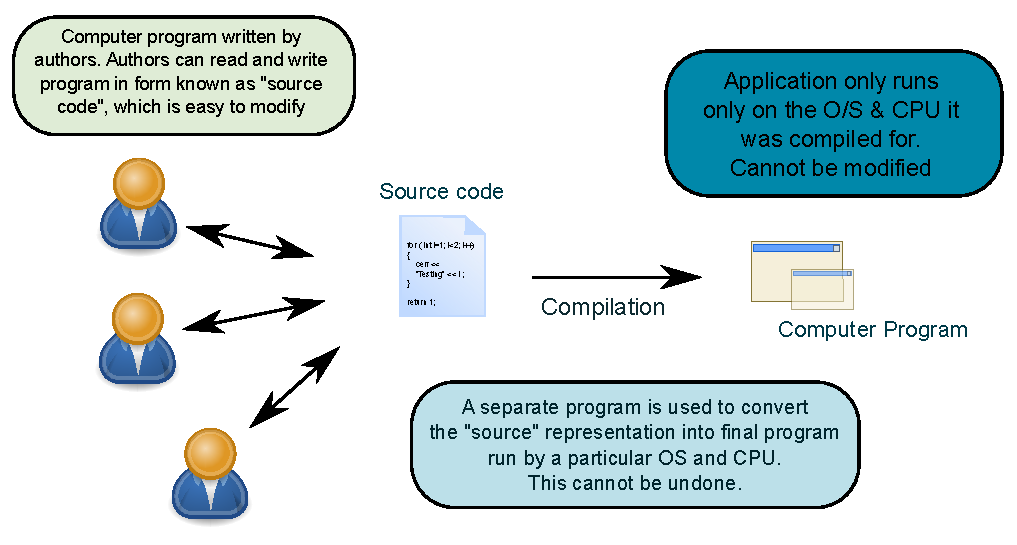
\includegraphics[width=0.7 \textwidth,keepaspectratio=true]{./figures/compilation.pdf}
 % camera.pdf: 578x382 pixel, 72dpi, 20.39x13.48 cm, bb=0 0 578 382
 \caption{Closed-source programs only provide the final application, are neither human readable nor modifiable, and will only work on a specific platform. By contrast open source programs distribute the source-code as well as the application. The source code is the core logic which can be made to work on many platforms due to the invariance of the program logic.}
\label{fig:compilation}
\end{wrapfigure}
Open source programs are programs which distribute not only the executable code, which is understood by the computer (so called machine code), but also provides the version of the program as it was written by humans as well. This provides external users with the possibility of modification or verification of the program behaviour, either by themselves, or by engaging a third party. With the source code one can verify the correctness of the system, alter behaviour or otherwise modify the program, or even reuse sub-sections of the program elsewhere. 

Modifications to the program itself may include migrating the program to newer or older systems, adding new functionality, or correcting errors in the program implementation.  
 
To provide the user with these capabilities, the program is distributed with a so-called \textit{libre} copyright licence. The program is distributed at no cost to the end user, and the copyright attached to the program explicitly allows modification and re-distribution (copying) of the program to other parties.

Note that there are restrictions on what may be done with the program, for example it is in violation of the licence to claim ownership of the program, or to use technical measures to prevent access to the program, or modification thereof. The licence used in the program is a generic one shared by many free (as in freedom) software programs. 

If you have been charged for this program, it is suggested that you request a refund and obtain a free copy from the main website, as listed on the front cover of this document. If you wish to have the full licence details (GNU General Public Licence Version 3 (or any later version)), please see the \texttt{COPYING} file distributed with this program. If this is not available, please see the project website, or perform an Internet search for the licence name.
 
\subsection{Requirements}
Due to the design of the program, the program should run under Linux, Mac, BSD and Windows machines. The program does not rely on CPU specific features, and thus should be able to be run under x86, x86-64, arm, or whatever. Basically, it should run just about anywhere. Every effort is expended by the author to ensure that the program can be run on as many devices as possible; if your platform is not supported, it may be possible for either you, or the author to generate executables for your system. See the section ``Getting Help'' for contact details.  

The minimum requirements for running \emph{3Depict} are not known. The author wrote a substantial portion of the program on a machine with only 4 and 12~GB drives, and a 1.6~GHz processor, which normally runs at 800~MHz and has 1~GB of RAM. There is no clear reason that it would not run on even lower-spec machines. Whilst a higher spec machine may run the program faster, intelligent use of the programs ``filter'' system may allow for complex analyses even on low-end machines. 

If you are experiencing 3D graphics problems, first ensure that other 3D programs do not experience the same problems. Otherwise, please contact the authors for assistance -- there should be no requirement for vendor-specific hardware. Note however that the exact appearance of the 3D view is dependant upon your hardware, and may have small changes between different platforms. 

\subsection{Platform specific notes}
Note that whilst every effort is made to ensure that the program will run on a variety of systems, small system-specific quirks may be evident, particularly on platforms to which the authors do not use regularly (\emph{e.g.}\ windows). Secondly, due to slight differences between platforms some functions may be remapped to other mouse/key combinations.  

Mac:
\begin{itemize}
 \item \texttt{Ctrl} keys may sometimes be mapped to the \texttt{Command} (clover) key.
\end{itemize}

Windows:
\begin{itemize}
 \item \texttt{Ctrl+Tab} cannot be used as a key combination, as this is reserved for switching between user interface elements. \texttt{Ctrl+Alt} is used instead.
\end{itemize}

 
\subsection{Getting help}

Assistance with this program may be freely obtained over the Internet at \url{http://threedepict.sourceforge.net}. Questions regarding use of the program, feature or bug reports will be attended to as soon as possible. Contact options include email (via the online web-form), or an online forum.

If the program crashes in a predictable manner (\emph{i.e.}\ you know how to trigger it), this is a bug and needs to be fixed. Please report the bug in this case, so we can fix it as quickly as possible. If the program crashes in an unpredictable fashion, please still report it as best you can, and we will try to fix it if we can isolate the problem from the description. For advanced users, we would appreciate backtraces, packages,  and any other relevant information in both of these cases.

\subsection{Who wrote this program?}

This program was written by D. Haley, in his spare time. A. Ceguerra provided  additional development from Version~0.0.2 and provided assistance with debugging and fixing the Macintosh version, and providing executable versions of the program for OSX in 0.0.1. 

\subsection{Alternate documentation}
For the more visually inclined, screencasts of the program have been created, and are available on the project website. These videos exhibit basic use of the program for various simple analyses. At time of writing, the only literature available for the program is this document, and the online screencasts. If you have questions, please contact us through the website, where we will reply as soon as possible. 

\subsection{Helping out}

\emph{3Depict} takes time to develop, and no doubt could be better than it is now. However, this doesn't all just magically happen -- people have to put the work in. Development time by the authors is split between testing the program, reproducing bugs, coming up with new ideas for program changes, editing documentation, making pretty pictures, maintaining websites, and even developing the program. 

We would always appreciate assistance with this work. You don't have to be able to write computer programs. For example, we would like to translate the program into other languages. If you can translate a spreadsheet table into another language, this is helpful. If you can work out what triggers particular bugs, this is  helpful. If you can improve this document, this is also really helpful. Of course, if you can program (C/C++) and are willing to help, grab a copy of source from our website contact the authors, because a little code goes a long way.

\section{Basics}
\subsection{Getting started}
\subsubsection{Licence}
\label{sec:licence} 
This program is distributed under the GNU General Public Licence Version 3 (GPLV3+), an \textit{open-source} licence. Information on the copyright of this program is available under the \texttt{COPYING} file in the program directory, or online (\emph{e.g.}\ \url{http://www.gnu.org/licenses/gpl-3.0.txt}).

The basic premise is that you may copy the program, modify and distribute such modified versions or derivative works only under the same licence. The licence forbids technical restrictions on users further redistributing the program.
 
\subsubsection{Installing the program}
The installation method for the program depends upon your chosen operating system. The most up-to-date notes are available on the project website. It is highly recommended that, in general, you do not simply download random programs from the Internet and execute them if a version is available in a trusted software repository. 

\subsection{Understanding the interface}
The program interface consists of three different views. On the left, there is the data, cameras and tools panes, with are used to generate data for visualisation, and to provide an interface into changing properties in a structured manner. On the right, the view is split into two sections; at the top, there is the 3D view. At the bottom are the plotting, raw data and console output panels.  

\begin{figure}[ht]
  \centering
 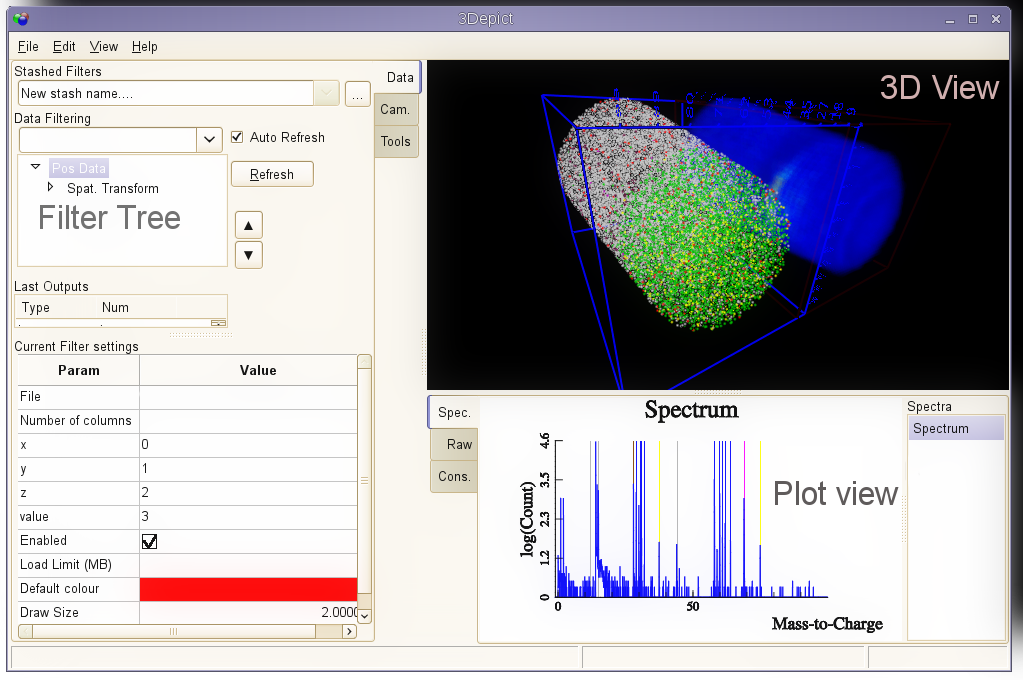
\includegraphics[width=0.85 \textwidth,keepaspectratio=true]{./figures/interface.png}
 % camera.pdf: 578x382 pixel, 72dpi, 20.39x13.48 cm, bb=0 0 578 382

 \caption{Interface layout. The 3D view, plot panel and filter tree are labelled.}
\label{fig:interfaceLayout}
\end{figure}


Each pane may be hidden, either by double clicking the ``sash'' between the two panes, by selecting the respective item from the view menu or by its keyboard shortcut key as listed in the menu.  

At the very bottom of the program, a status bar is shown -- here messages are shown to provide hints on how to use the program, or to communicate information relating to the program's internal state. 


\FloatBarrier
\subsubsection{The 3D View}

The 3D view is used to show the three-dimensional objects generated during a data analysis, and provides a direct method of interaction with the 3D Scene. Through the use of the mouse (or other pointing device), the 3D view can be manipulated to change the view position and orientations. Some objects in the 3D view are interactive, and will be indicated by an overlay in the top right of the window when the pointer is on top of such an object. 



\paragraph{Basic movement}
\begin{figure}[ht]
\centering
 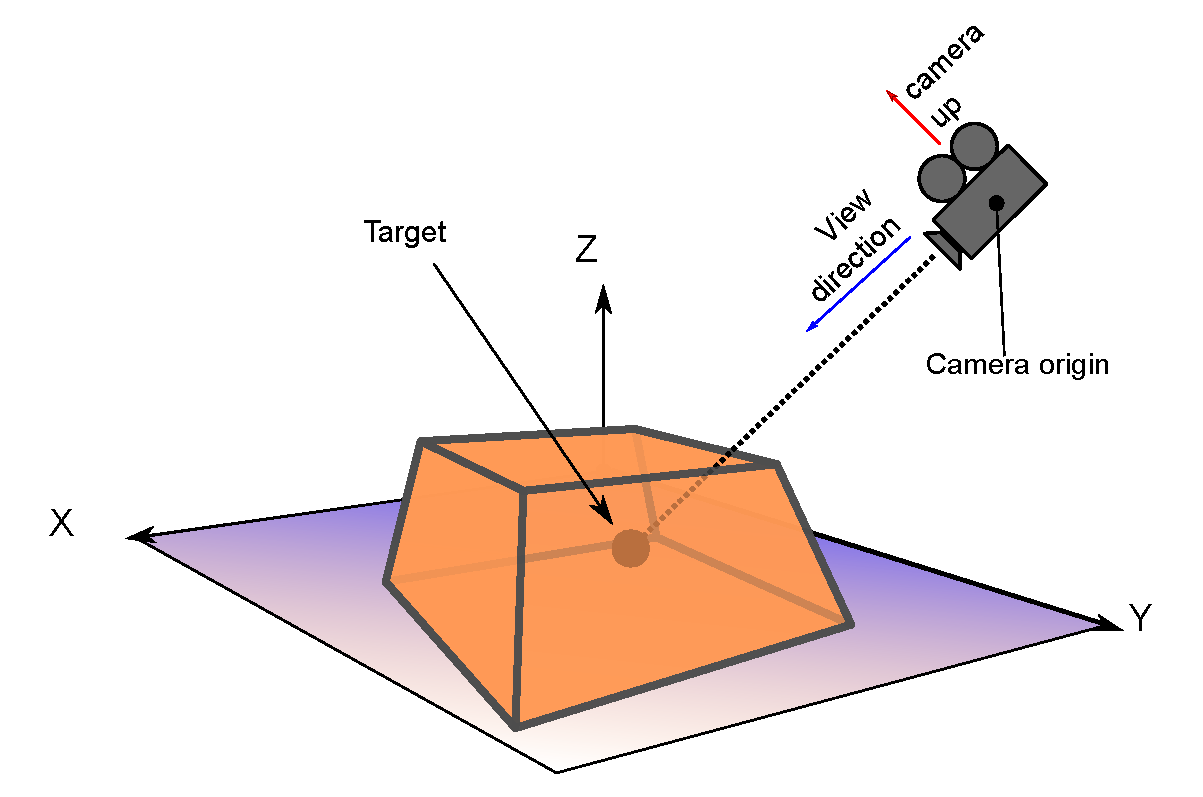
\includegraphics[width=0.7 \textwidth,keepaspectratio=true]{./figures/camera.pdf}
 % camera.pdf: 578x382 pixel, 72dpi, 20.39x13.48 cm, bb=0 0 578 382

 \caption{Basic camera layout. Each camera has a position, an up direction and a target. The 3D view is as seen by the camera. Cameras may be saved and recalled to return to specific views. Try to realise it is not the object that moves, but rather yourself.}
\label{fig:camera-basics}
\end{figure}
The 3D view represents your camera into a 3D scene of your construction; it is by manipulation of cameras that the view is interacted with; so you may zoom, orbit, pan, roll or swivel the camera view. If you are lost at any time, you may reset the view by tapping the space bar. To change the axis along which the view is reset, hold the \texttt{Ctrl} or \texttt{Shift} buttons whilst resetting.  Double tapping the space bar will cause the axis to be viewed from the reverse direction.

The basic 3D view consists of a ``target'' based camera, so when you move the camera, the camera will orbit around this target. To interact with a scene, hold down the left mouse button and move the mouse to control the camera.  


The basic keys for controlling the camera move mode (left click) are\footnote{As stated previously, mac systems do not use the Ctrl key.}:  
\begin{itemize}
\item  \textbf{No key}: Orbit camera 
\item \textbf{Ctrl}: Pan camera 
\item  \textbf{Tab}: Swivel camera (Look about)
\item  \textbf{Ctrl +Tab} (Windows \textbf{Ctrl+Alt}): Roll camera around viewport centre. Note that the rolling motion is controlled by the position of the mouse click.
\item \textbf{Space/Shift+Space/Ctrl+Space}: Reset camera bounds and position to look along X,Y or Z axes respectively.
\item \textbf{+/-}: Zoom in/out.

\end{itemize}
For any motion, the \texttt{Shift} key may be used to increase the camera move speed.  Scrolling on the window zooms in or out. For a perspective camera, zooming is performed by moving the camera closer to the object. For an orthographic camera, zooming simply scales the view, whilst holding the camera position constant.


\subsubsection{Plot area}
The available plots are listed on the right hand side of the plot view panel. You can select the active plot from the list. The items in the list take their name from the filter from which they originates name (there are exceptions to this rule, \emph{i.e.}\ composition profiles). Several plots may be drawn at once by holding down the \texttt{Ctrl} key when selecting the plot to draw from the plot list box.  


\begin{figure}[ht]
\centering
 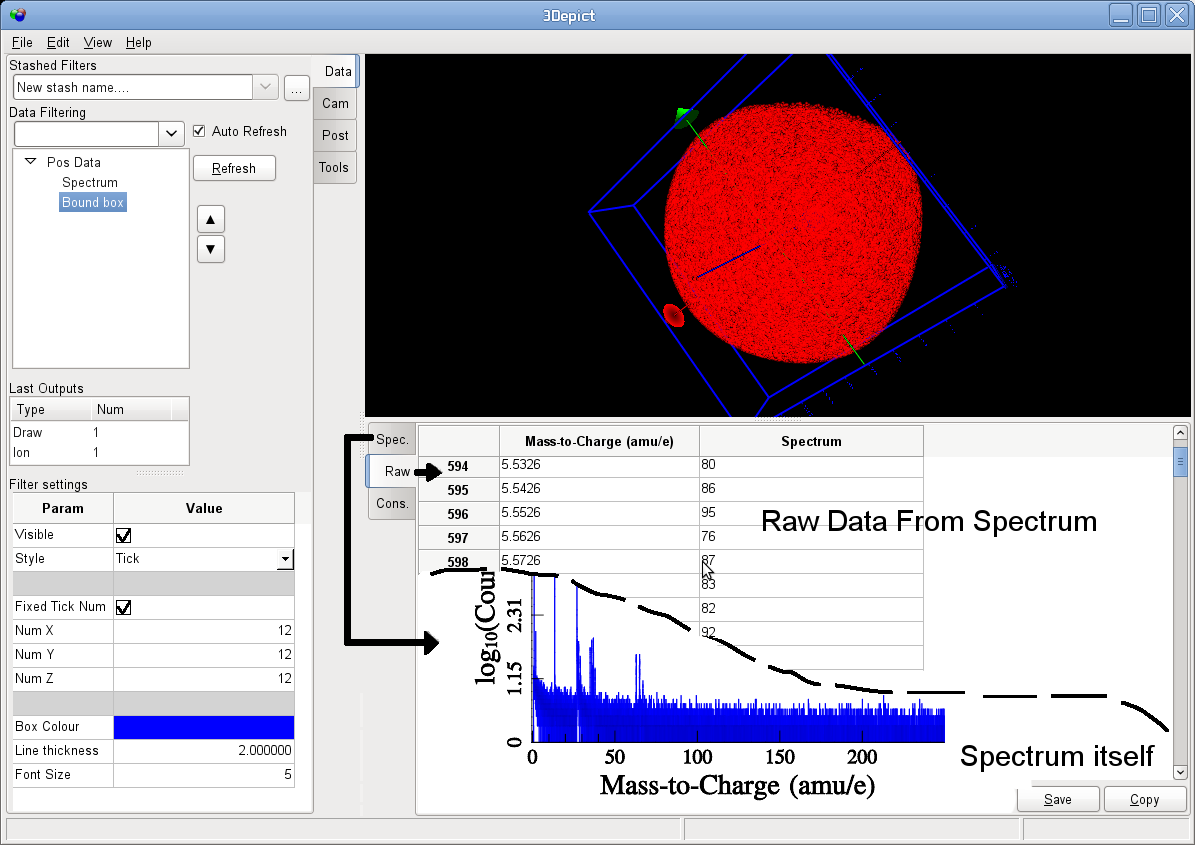
\includegraphics[width=0.85 \textwidth,keepaspectratio=true]{./figures/spectrum-raw.png}
 % camera.pdf: 578x382 pixel, 72dpi, 20.39x13.48 cm, bb=0 0 578 382

 \caption{Raw data pane, with associated spectrum displayed. Data can be selected, and saved for external manipulation as desired.}
\label{fig:raw-basics}
\end{figure}


Raw data is visible in the ``raw'' tab (Figure~\ref{fig:raw-basics}), and will show the output data from the selected plots, with the axis labels for each plot. The data can be saved to a file from this view.



\subsubsection{Console}
Each filter may optionally generate console output. In the case, a text area will contain messages from the filter to the user. An example of the messaging area, and the messages are displayed in Figure~\ref{fig:console-basics}. As can be seen in this figure, if a message has been generated from a filter, but is not the messaging area is not active, the console tab will display a small marker to denote new messages pending for review. The exact marker that is shown is dependant upon the operating system.

\begin{figure}[ht]
\centering
 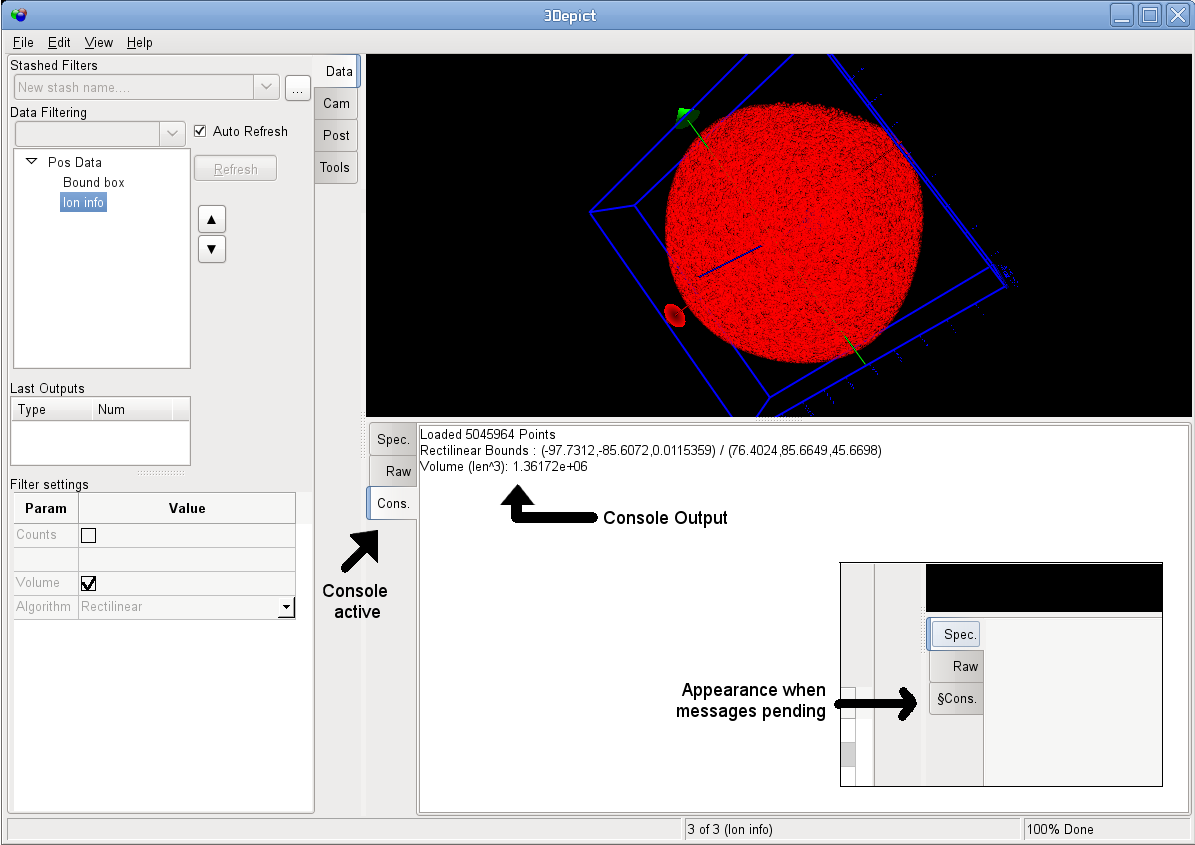
\includegraphics[width=0.85 \textwidth,keepaspectratio=true]{./figures/console.png}
 % camera.pdf: 578x382 pixel, 72dpi, 20.39x13.48 cm, bb=0 0 578 382

 \caption{Console tab, with sample console messages. The inset shows how the tab will appear if messages are pending whilst the console itself is hidden.}
\label{fig:console-basics}
\end{figure}


\subsubsection{Tools panel}
The tools panel offers several options on changes to the way the program operates internally. 

\begin{itemize}
\item  \textbf{Smooth and Translucent objects}: This enables so-called ``alpha blending'' in the 3D scene, where appropriate which allows for non-opaque objects, and anti-aliased objects. This mode alters the way in which objects are rendered in the 3D scene and is in effect a quality-appearance tradeoff. Most of the time you will probably want it set to ON. The program may render the 3D scene slightly faster if this is disabled.
 
\item  \textbf{Enable lighting}: 3D objects do not look very 3D if you are only seeing them on a 2D screen. Computer graphics works around this by simulating the effect of having a 3D lighting source. This might provide minor performance improvements if disabled, at the cost of clarity of rendering.
 
\item \textbf{Enable filter caching}: This alters the way in which the program processes the filter tree. Normally, the program performs what is known as a depth-first search, and propagates data generated by the program from one filter to the other. Intermediate copies are kept by the filters themselves to speed up recomputation. However, this strategy has a large downside, which is memory consumption. Disabling this will reduce memory consumption by filters, but will mean that any change to the filter tree, no matter how small, will cause the entire tree to be recomputed, including data loading.

\item \textbf{Weak and fast random}: This setting is a program wide setting that switches the strength of the random number generator. However, for more robust statistical results, it is recommended that this be disabled when computing final values. When enabled, the program will use a Linear Shift Feedback Register using a maximal length Galois polynomial to generate numbers required for random sampling. This has the advantageous property of being a somewhat random entirely non-repeating sequence that is fast to generate, but having sufficient decorrelative strength against most inputs to provide the appearance of random sampling. 
\end{itemize}


\subsection{Usage fundamentals}
Initially the program window will appear with only the default world axes visible. To provide a more interesting view, it is necessary to inject data into the program.  To do so, select the File menu, and then select using ``Open''. At time of writing, only two formats are currently supported. Firstly are ``POS'' files, and secondly are text files, each which consist of X,Y,Z and a values (usually mass-to-charge)\footnote{For a technical description of the POS file format see Section~\ref{sec:posformat}. For a description of suitable text formats see~\ref{sec:textformat}}. To load a file, navigate to an existing POS file on your disk. If you do not have a POS or text file, small example files are available on the project website, on the documentation page.  

Upon selecting the file and then \texttt{Open}/\texttt{OK}, the file will be loaded into the viewport. Note that the entire file is not loaded, but rather a random selection of elements in the file. 

Loading this file populates a small treeview on the data pane (at the left). This tree is referred to as the ``analysis'' tree, and each item in the tree is called a ``filter''. The tree is responsible for producing the output data in the scene, and a good understanding of the behaviour of this tree is required to extract the maximum benefit from the program. Each item in the tree has a list of properties that can be modified. For example, the amount of data loaded by the ``pos load'' filter can be altered by selecting the ``pos load'' item from the tree, then in the grid below, entering in the new amount of data to load (you can set this to 0 to load the entire file). 

Thus, each filter can be individually altered to change its behaviour. However, each filter acts upon the output of the filter that is a ``parent'' to it (in the case of not having a previous filter, each filter will act as if it had no incoming data). Thus the arrangement of each filter in the tree is critical to the output of the program. In order to modify the  layout of tree, you may add new and move, copy or remove existing components of the tree.  Changes to the tree, or any filter contained therein, may be undone using the ``Undo'' menu item, or with the keyboard shortcut \texttt{Ctrl-Z}.  Each filter's behaviour is outlined in Section~\ref{sec:filter}. More information on the tree behaviour is given in Section~\ref{sec:treebehaviour}.

Note that with every modification of the tree, the 3D scene and any plots will be recomputed. The time of computation is dependent upon the amount of data that is to be analysed, and can be reduced through sampling or volume restriction methods. By default, each filter may cache its own output, in order to speed repeated computations.

To delete an item, simply select the item to delete with the mouse, and then use either the \texttt{Delete}  or  \texttt{Backspace} keys on your keyboard. Note that clicking on an already selected item will activate the name edit mode. To exit this mode, press \texttt{Escape}. 

New items can be added to the tree by selecting the filter to add from the dropdown box immediately above the tree. When selecting a new filter to add; an element in the tree must be selected, where the new filter will be placed. If there is no item selected, an error will be shown in the status bar.  

Once an item is added, the filter tree is thus modified and a recomputation of the scene will occur. Approximate progress on the filter update is visible in the status bar. During an update, only limited interaction with the program is permitted. An update may be cancelled at any time with the \texttt{escape} key. 





\section{Understanding the program}
\subsection{Filters}

Filters form the key component of the program. These are the tools by which data is analysed and modified, in order to generate the visual representation that is needed by the end users. The basic idea behind a filter is that each filter may perform arbitrary operations on ``data streams''. These data streams are sent to and from each filter, flowing through the tree.

\begin{figure}[htp]
 \centering
 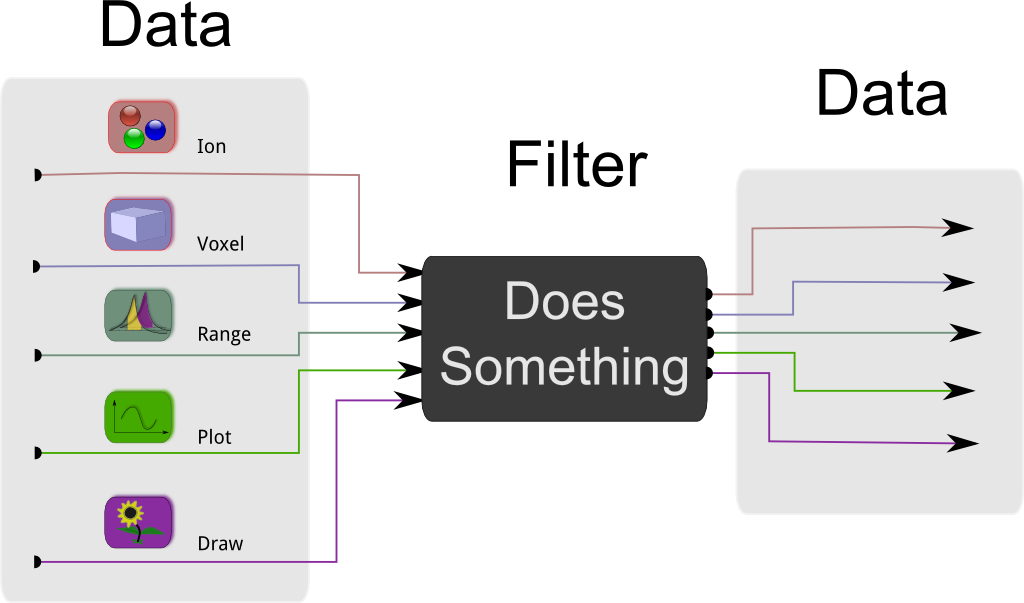
\includegraphics[keepaspectratio=true,width=0.85 \textwidth]{./figures/generic-filter.png}
 % generic-filter.png: 10x603 pixel, 17dpi, 153.75x90.54 cm, bb=0 0 4358 2567
 \caption{Basic concept of a filter. Data goes in, data comes out. The filter may perform any operation on the data coming in or out as it chooses. The data streams coming in are restricted to certain types of data, as shown. }
\label{fig:basic-filter}
\end{figure}


The basic idea of a filter is illustrated in Figure~\ref{fig:basic-filter}. \emph{3Depict}'s flexibility is that these filters can be arranged in any way that makes sense to the end user. There is no restriction on placement of filters -- some placements may be totally useless, others may be exceedingly useful. It is up to the creativity of the end user to determine whether any single arrangements meets their needs.

\subsection{Trees}
\label{sec:treebehaviour}
The tree is a flexible and powerful system for constructing your own analyses, after some use this will become a familiar and readily modifiable system for performing your analyses, however the initial structure of the program may take some getting used to. If you are familiar with programs such as \emph{Paraview}, you may already be familiar with this concept.  

The filter tree essentially is a system for injection, manipulation and display of the data in the program. The tree becomes an ``assembly line'' for the view of data in the 3D and plot views.  The nodes of the tree are the filters that act on or insert data into the analysis. Each node in the tree may be considered in what is called a ``parent-child'' relationship. Each element in the tree (except the first) has a ``parent'', and thus may have their own ``child'' elements. Each ``parent'' may, in fact, have many children. Data may be considered to propagate from the ``root'' of the tree downwards, with each filter in a direct line somehow modifying the data from above in some way. When data reaches the end of the filter tree it is ``picked up'' by any of the 3D view, plot or console panels, depending upon the nature of the data. 	

The basic method for data flow is that a parent gives a copy of the data it has processed to its ``children'' to modify in some way. Each ``child'' has its own copy\footnote{Technical note: the ``copy'' system is at the discretion of each filter. Child filters are given a reference to the parent data which restricts modification of the parent's data by the children; children may or may not duplicate this data, propagate or terminate the reference.} of the data from the parent, which it modifies. In turn this child then gives a copy of the data to each of its own children. If a filter has no children it then passes the data to either the 3D view, the plot view or the console view, depending upon the data type.  

\begin{figure}[ht]
 \centering
 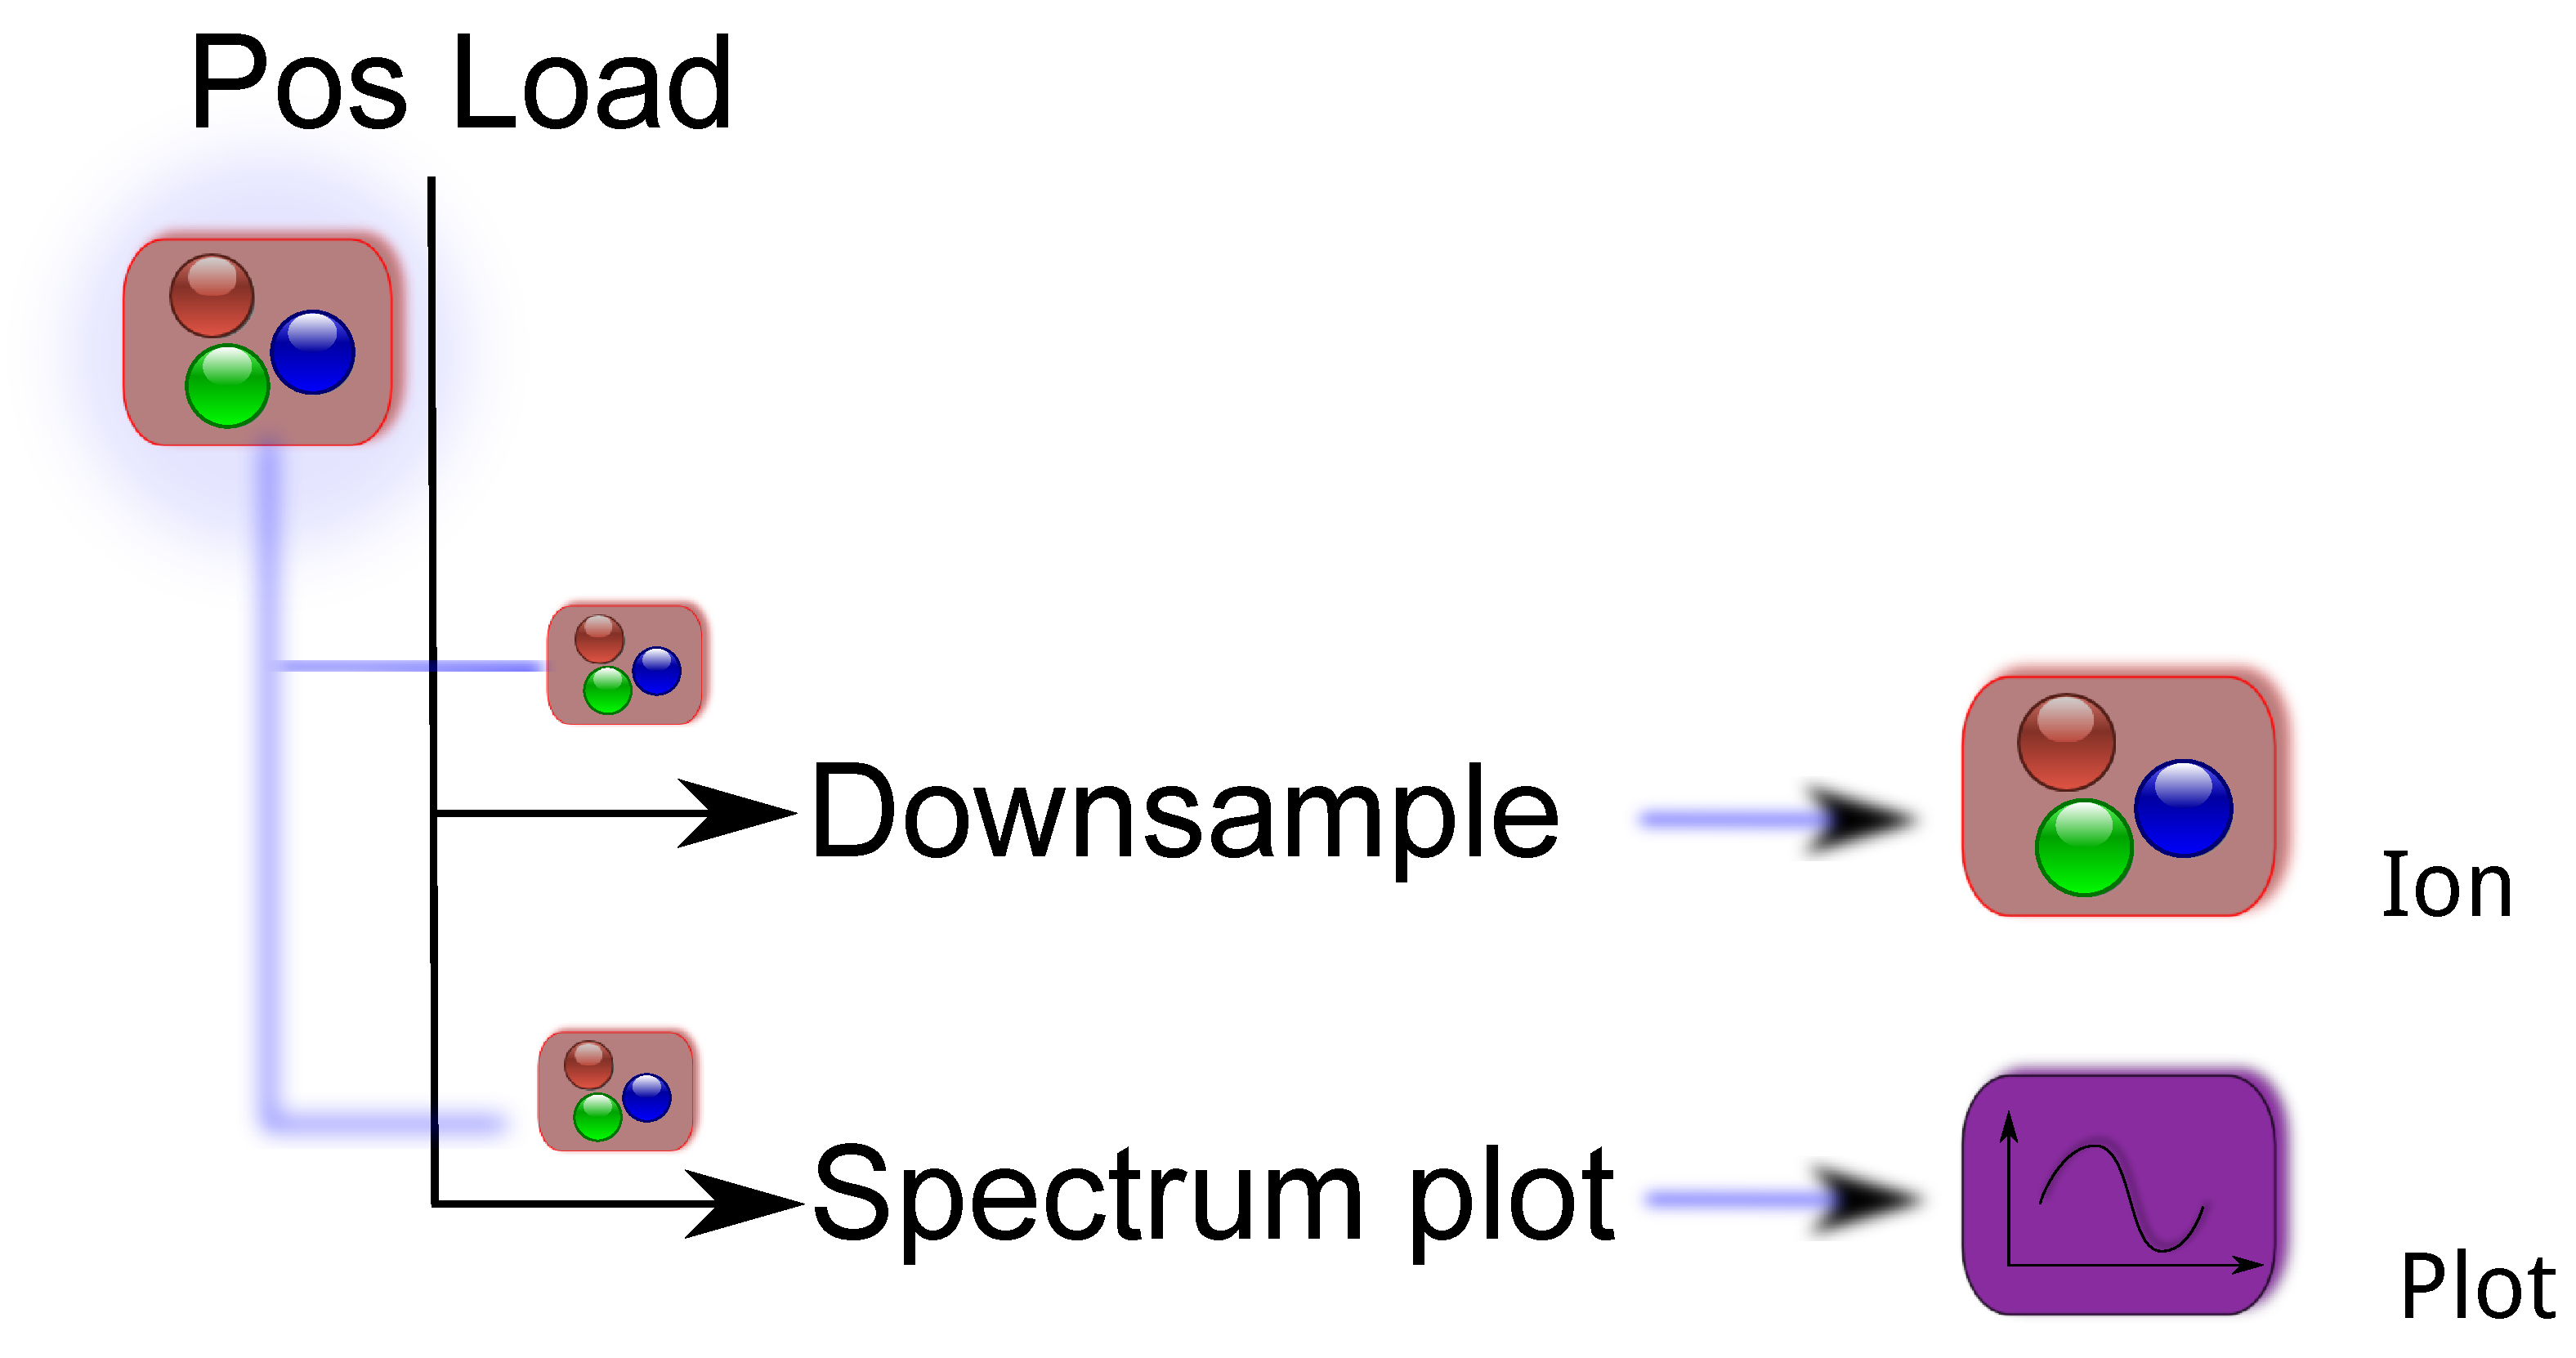
\includegraphics[width=0.85 \textwidth]{./figures/tree-propagate.pdf}
 % tree-propagate.pdf: 1513x798 pixel, 72dpi, 53.38x28.15 cm, bb=0 0 1513 798
 \caption{Data propagation in a tree for a particular arrangement of filters. Data is propagated from a parent filter to its children.}
\label{fig:datapropagate}
\end{figure}


Using this method, one may create a variety of different analyses; for example, one may wish to subsample data before performing a time-consuming spatial analysis, or one may wish to clip the data to remove unwanted sections before generation of a value spectrum. The flexibility of the filter system supports this concept.

Note that items in the filter tree can be moved. You may move any filter to a new parent by dragging with the mouse. In order to copy instead of move, hold down the \texttt{Ctrl} whilst moving to duplicate the filter, rather than moving it.  

You may also rename filters in the tree; The filter name may be used by the filter to generate its output, \emph{e.g.}\ spectrum plots will take the plot title from the filter name. 



\subsection{Stashes}

Instead of enabling or disabling sections of the tree, the program supports ``stashes'' as a place to put sections of the analysis tree for later use without using them in the analysis section. To create a ``stash'', select a section of the filter tree to ``stash'', then in the ``stashed filters'' dropdown on the data tab, type the name of the stash you wish to create (this is up to you), and press \texttt{Enter}. Once done, a duplicate of the subtree specified (\emph{i.e.}\ all the filters below the selected one, and the selected one too), is made. This process is shown in Figure~\ref{fig:stash-creation}. You can view the contents of the stash by selecting the button next to the stash dropdown, and you may delete stashes however you cannot edit them.  


\begin{figure}[ht]
  \centering
 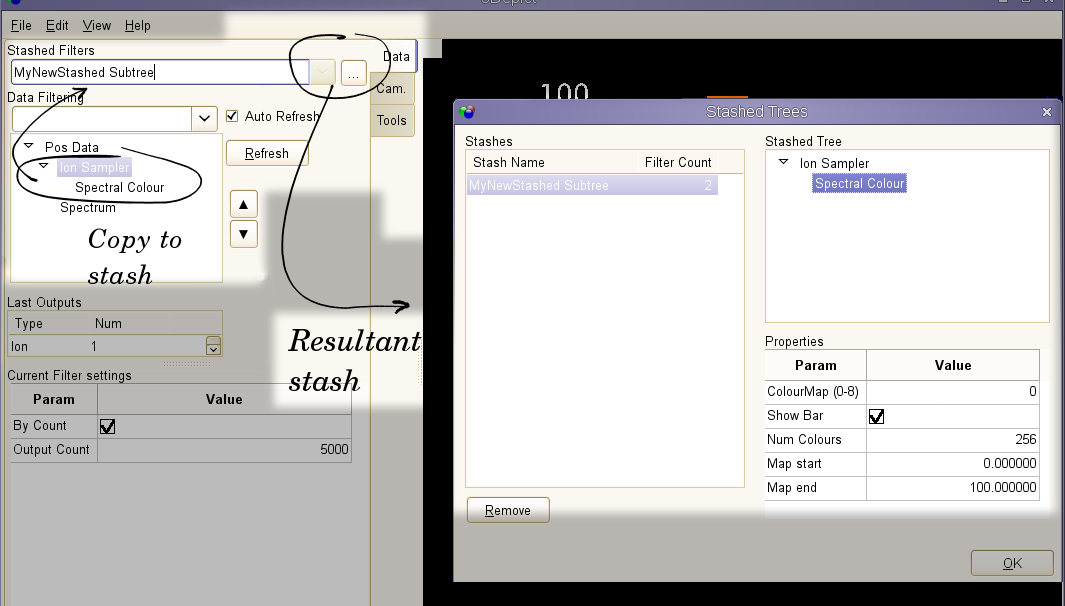
\includegraphics[width=0.85 \textwidth,keepaspectratio=true]{./figures/Stash-operation.png}
 % Stash-operation.png: 1065x606 pixel, 72dpi, 37.57x21.38 cm, bb=0 0 1065 606 
 \caption{Creating a stash from the filter tree. New stashes will appear in the dropdown and can be selected to recall subtrees to insert into the filter tree.}
\label{fig:stash-creation}

\end{figure}

To use a stash, select a filter in the tree and then click the dropdown button on the stash combo box, and then select the stash you wish to use. This will place the stash as a child of the selected filter. Note that the stash can be used multiple times.  

\subsection{Plots}
Any plots generated by the filter system are displayed in the plot pane. It is possible to zoom or pan the view as required by dragging or \texttt{shift} dragging the plot respectively. Double-clicking the plot returns the plot back to its original scaling.

The associated numbers used to generate the selected plots are shown in the ``Raw'' tab. Note that plots can contain ``regions'', such as generated by a range file. In this case, each region may be manipulated in-situ, by dragging the regions sides, or its centre to alter or move the region respectively. These modifications will be propagated back to the original filter.

Each plot is either logarithmic, or linear in scaling. Mixing these two types of plot will result in the y-axis stating that there are mixed data types in the plot. The log/linear mode is determined by the filter that generates the plot. Note that due to internal limitations (fixed plot palette in the underlying library), the colours observed in the plot may be slightly different from those specified by the filter.

\subsection{Cameras}
To fully understand the camera model, it is necessary to understand the parameters in the camera property tab. Initially there is only the default camera, which is unnamed. By entering in a name for the camera, you can access the properties for that particular camera. By entering in more names, you can create multiple cameras, saving the position of existing cameras as you go. This can allow you to jump between different camera views as desired.

One can select the position of the camera, a position that the camera is always looking at (target), the camera ``up'' direction, and the field of view. Furthermore, the camera type (perspective or orthogonal) can also be selected.

With the exception of the field of view, these parameters are dynamically modified when interacting with the 3D scene (see section X). The camera field of view, however requires special mention. The field of view of the camera is the angle that the camera look at. Human vision is around 120*, and is much narrower for suffers of tunnel vision (say, 30*). A bird has a full 360 degree field of view (it can see in all directions without needing to turn its head). By default the camera is set to 90*. To get the ``fish-bowl'' effect, where close objects appear very large, this number can be increased. To get an effective orthogonal camera, this number can be set very low. Note that changing this value will also have the apparent effect of zooming the camera in or out, so tapping \texttt{space} to reset the camera view is recommended for large changes. 

\subsection{Effects}
The effects tab allows for altering the appearance of the 3D output data, without changing the data itself. Current effects are anaglyphic 3D (colour-based 3D glasses), and visual clipping.  

\subsection{Program actions}

\subsubsection{Save}
The current programs state can be saved to an ``XML'' state file for later analysis\footnote{See Section~\ref{sec:xmlstatefile} for more information.}. Note that opening an existing program state file will erase your current state. If you wish to merge the two states together into a single analysis, use the ``merge'' option. Note that as this file references, but does not contain, the data files needed for the analysis, this file cannot be moved between computers and expected to ``just work''. However, to overcome this, the program provides the ability to export an analysis ``package'', which contains all the data necessary to move these files between computers with ease, regardless of platform. This feature is explained in the ``Export'' section.

\subsubsection{Undo}
The program has an undo feature which can be used to abort the last changes to the filter tree. Note that for memory reasons, the results of the computation are not stored, and will need to be recomputed. Note that there is also a ``redo'' function, which allows for undone changes to be restored. 

\subsubsection{Raw Data}
The raw data pane may be used to obtain the raw XY data used to generate the plots. This can either by copied and pasted, or alternately saved to file.  

\subsubsection{Export Menu}
Plots, images and ion data may be exported from the program. The output format for 3D images is the ``Portable Network Graphic (PNG)'' format; these are supported by almost all image viewers. 

For plots, you may save in either (Scalable Vector Graphic (SVG)) or ``PNG'' forms. Note that due to the nature of the SVG files, no resolution is needed, and the image can be reproduced at any scale. Furthermore the SVG can be used later to generate PNG images at the required size for output (We recommend the program \textit{Inkscape}). Alternately saving as PNG can be done, and you will be prompted for the desired image size.

Exporting Ion data can be done in several ways; you may export only the visible ions, or alternately, you may export only a subset (for example one or two ranges) of the data, depending upon the filter that the data emerged from (\emph{i.e.}\ per leaf filter). The output format will be in Big-endian ``POS'' format, as  detailed in the Appendix, Section~\ref{sec:posformat}.

Modified range files may be exported in whole. Currently the only supported export format is the oak-ridge``RNG'' format

Simple animations of the 3D data can be constructed, where the current camera is orbited 360 degrees around its target location. The result is saved as an image sequence, which can be converted into an AVI using programs such as \emph{ImageJ}, or \emph{ffmpeg} to convert the constructed image sequence into a video file.

Finally one can export the entire analysis state, including all required data using the export analysis package option. This will create  a folder which contains all the files needed to reproduce the current program state elsewhere. Note that this imports all referenced data files, so the package can become quite large, but should be fully portable to any other system by simply copying the created folder. Inside the folder, the program state will be stored as a state file, and can be accessed by simply opening this state file.

\subsubsection{Autosave}
The program will generate an autosave file periodically. If the program crashes, it will look for an autosave file and prompt you to restore it. Note that only the program settings are saved, not the intermediate data, so recomputation will be necessary. If the autosave fails to load, then the autosave file will be archived; in this case, please consider sending the failed file to the developers.


\section{Detailed Reference}
\subsection{Data types}
Different data can propagate through the filtering system before it is seen in the 3D view. The currently available types are ions, plots, range, voxels and drawable object types. Although these are used internally by the program, understanding the type system may enable more advanced use of the program. If you are not interested in this, skip to the next section.  

\subsubsection{Ions}
Each ion represents a point in space, which has a value type associated with the point. For example, one might consider a point in a dataset where positions represent atomic positions, and the value is the measured atomic mass. Ions are grouped together by different filters, and each group may be represented with a unique colour and size.  

\subsubsection{Plots}
Plots can be passed between filters to allow for a 2D graphical representation of whatever it is that the filter computes. Plots are a X-Y paired set of scalar values, which are finally given a visual representation as a plot. Plots have a title, and a label, and may represented either on a linear scale, or a logarithmic one.

\subsubsection{Range}
This is a special datatype which propagates information through the filter tree. The data represents non-overlapping regions of the value space which are to be tagged as belonging to a certain group. This data type has no actual output into the 3D scene, but can alter the manner in which ``downstream'' filters process incoming information. For example, if a profile filter is used after a range, it will split up its measurements into a per-tag ``range'' section. 

\subsubsection{Voxels}
Voxels is shorthand for ``volume pixel'' and is a rectilinear region of space, divided up into an equally spaced rectangular grid. Voxels can currently be represented by a point cloud, where each point has a given colour and transparency, or by a triangulated surface (an iso-surface) which represents the contouring surface for a given scalar value.

\subsubsection{Drawables}
3D primitives can be injected into the data stream to assist in the final representation of the scene. Items such as spheres, lines triangles or text can be placed in the final scene.
 

\subsection{Filters}

In this section, the detailed behaviour of the various filters available in \emph{3Depict} is outlined. Recall that each filter interacts with other filters and the visualisation environment by generation and propagation of various filter types. At the most abstract level, there are three ways that filters can interact with the data -- the list given below provides a may (optional) or will (guaranteed) output.

\begin{itemize}
 \item \textbf{Emit:} Emitting a new data stream into the filter output (Yes: filter may emit, No: filter will not emit).
 \item \textbf{Use:} Using a new data stream for internal calculations (Yes: filter may use, No: filter will not use). 
 \item \textbf{Block:} Preventing an incoming stream from propagating to the output (Yes: filter will block, No: filter will not block).
\end{itemize} 

This section describes each filter in turn, the fundamentals of the internal computation, and provides a table describing which datastreams are emitted, used or blocked during the filter's refresh cycle.

\label{sec:filter} 
\subsubsection{Data load}
 
The data load filter injects 3D point+value data into the analysis tree. Points are loaded from a file by one of several different methods. By default, random data is selected from the file. This filter can be created using the ``load'' function from the file menu. Note that the default settings will only load a random subset of the data in order to speed analysis. If you require all data to be loaded, then you will need to alter the filter settings. 
\begin{itemize}
\item  \textbf{Number of columns}: Number of floating point values in a single record. Defaults to 4.
\item  \textbf{X}: Position in record to use as X value. Defaults to 0.
\item  \textbf{Y}: Position in record to use as Y value. Defaults to 1.
\item  \textbf{Z}: Position in record to use as Z value. Defaults to 2.
\item  \textbf{Value}: Position in record to use as associated scalar value. Defaults to 3.
\item \textbf{Enabled}: Disable/enable the filter.


\item \textbf{Monitor}: Monitors the timestamp of the input file for changes -- if the timestamp on the file changes, then the data file will be reloaded, and the filter tree refreshed. This is useful when generating data files programatically.
\item  \textbf{Ion colour}: Colour of the ions from the 3D view.
\item  \textbf{Ion size}: Default size of points in 3D view.
\item  \textbf{Filename}: name of the file to load the data form.
\item  \textbf{Load limit}: The maximum quantity of data to load from the file. If set to 0, then the entire file is loaded. Otherwise a random sub-selection of the file is loaded. Note that random selection reduces memory cost, but if it is more than a few percent of the file size, may be slower to load. 

\end{itemize}

Information on acceptable data file formats is provided in the Appendix, in Sections~\ref{sec:posformat} and~\ref{sec:textformat}.

{%
\newcommand{\mc}[3]{\multicolumn{#1}{#2}{#3}}
\begin{table}[!Htb]
\caption{Propagation matrix for Data load.}

\begin{center}
\begin{tabular}{llll}
\hline
\mc{1}{c}{\textbf{\underline{Stream}}} & \mc{1}{c}{\textbf{\underline{Emit}}} & \mc{1}{c}{\textbf{\underline{Use}}} & \mc{1}{c
}
{\textbf{\underline{Block}}}\\
\hline \\ [-2.2ex]
Ion & Yes & No & No\\
Plot & No & No & No\\
Drawable & No & No & No\\
Range & No & No & No\\
Voxel & No & No & No \\
\hline 
\end{tabular}
\end{center}
\end{table}
}%

\pagebreak
\FloatBarrier
\subsubsection{Downsampling}

Randomly samples ions from the input stream. Can operate either to generate a fixed number at the output, or to take a fixed percentage of the input. If range information is provided, this can be done on a per-species level.

\begin{itemize}
\item  \textbf{Fraction}: Approximate random fraction of the data to load. Must be between [0,1].
\item  \textbf{Max count}: The approximate number of ions to load.
\item  \textbf{By count}: Specifies whether to use a fixed count, or a fixed fraction

\end{itemize}

{%

\newcommand{\mc}[3]{\multicolumn{#1}{#2}{#3}}
\begin{table}[!h]
\caption{Propagation matrix for Downsampling.}

\begin{center}
\begin{tabular}{llll}

\hline
\mc{1}{c}{\textbf{\underline{Stream}}} & \mc{1}{c}{\textbf{\underline{Emit}}} & \mc{1}{c}{\textbf{\underline{Use}}} & \mc{1}{c
}
{\textbf{\underline{Block}}}\\
\hline \\ [-2.2ex]
Ion & Yes & No & Yes\\
Plot & No & No & No\\
Drawable & No & No & No\\
Range & No & If available & No\\
Voxel & No & No & No \\
\hline 
\end{tabular}
\end{center}
\end{table}
}%

\FloatBarrier
\subsubsection{Ion Information}

This filter allows for the computation of ion counts in any input streams, as well as volume estimation. If a range stream is present in its input, (\emph{i.e.}\ a Ranging is a parent of this filter) then the filter will perform per-species computation of the value.

\begin{itemize}
 \item \textbf{Compositions}: Enable computation of the number of numbers of different ions (if ranged), or total ions in the input streams.
 \item \textbf{Normalise}: Normalise the composition values. This only has an effect if there is a range input stream.
 \item \textbf{Volume}: Enable estimation of the volume of space occupied by the ion streams. There are several algorithms for doing this:
    \begin{itemize}
	\item \textbf{Rectilinear volume}: Computes the volume of the minimal axis aligned rectangular prism, or bounding box, that can hold all the points in the input stream. Except for truly spherical datasets, the reported value will be a function of the data orientation.
	\item \textbf{Convex hull}: Computes the volume of the minimal convex enclosing polygonal object, known as the convex hull. This is parameter free, but may cause gaps in the data to be estimated as part of the volume.
    \end{itemize}
    
\end{itemize}

{%
\newcommand{\mc}[3]{\multicolumn{#1}{#2}{#3}}
\begin{table}[!h]
\caption{Propagation matrix for Ion Information.}

\begin{center}
\begin{tabular}{llll}
\hline
\mc{1}{c}{\textbf{\underline{Stream}}} & \mc{1}{c}{\textbf{\underline{Emit}}} & \mc{1}{c}{\textbf{\underline{Use}}} & \mc{1}{c
}
{\textbf{\underline{Block}}}\\
\hline \\ [-2.2ex]
Ion & No & Yes & Yes\\
Plot & No & No & Yes\\
Drawable & No & No & Yes\\
Range & No & Yes & Yes\\
Voxel & No & No & Yes \\
\hline 
\end{tabular}
\end{center}

\end{table}
}%
\FloatBarrier
\subsubsection{Ranging}
\label{sec:rangeFilter}

This allows for the cropping and segregation of ions in 3D space by their scalar values.

Each range loaded from the file may be enabled, either at the ion level (groups of ranges) or at the range level. The range values may be altered; however these may not overlap at any time. Note that these can be edited graphically (to some extent) if used in a mass spectrum. At time of writing, \emph{3Depict} cannot be used to generate range files, only write them.

\begin{itemize}
\item \textbf{Filename}: This is the name of the file to use as the range source. So-called ORNL ``rng'' files, Cameca ``env'' files and Imago/Cameca ``RRNG'' files are accepted. For information on the accepted file formats, see the Appendix, Section~\ref{sec:rangeFormat}.
\item \textbf{Drop unranged}: This causes any ions not ranged to be silently dropped from the filter output. This is best enabled for 3D viewing, and best disabled for spectrum plotting
\end{itemize}

{%
\newcommand{\mc}[3]{\multicolumn{#1}{#2}{#3}}
\begin{table}
\caption{Propagation matrix for Ranging.}

\begin{center}
\begin{tabular}{llll}
\hline
\mc{1}{c}{\textbf{\underline{Stream}}} & \mc{1}{c}{\textbf{\underline{Emit}}} & \mc{1}{c}{\textbf{\underline{Use}}} & \mc{1}{c
}
{\textbf{\underline{Block}}}\\
\hline \\ [-2.2ex]
Ion & Yes & Yes & Yes\\
Plot & No & No & No\\
Drawable & No & No & No\\
Range & No & No & Yes\\
Voxel & No & No & No \\
\hline 
\end{tabular}
\end{center}
\end{table}
}%

\FloatBarrier

\subsubsection{Bounding Box}
The bounding box creates a 3D box surrounding any point data in the input stream. The box uses relative coordinates, and has a specifiable font size, colour and line thickness. Several styles of bounding box may be chosen from a predefined list.

{%
\begin{table}[!h]
\caption{Propagation matrix for Bounding Box.}
\newcommand{\mc}[3]{\multicolumn{#1}{#2}{#3}}
\begin{center}
\begin{tabular}{llll}
\hline
\mc{1}{c}{\textbf{\underline{Stream}}} & \mc{1}{c}{\textbf{\underline{Emit}}} & \mc{1}{c}{\textbf{\underline{Use}}} & \mc{1}{c
}
{\textbf{\underline{Block}}}\\
\hline \\ [-2.2ex]
Ion & No & Maybe & No\\
Plot & No & No & No\\
Drawable & Maybe & No & No \\
Range & No & No & No\\
Voxel & No & No & No \\
\hline 
\end{tabular}
\end{center}
\end{table}
}%

Note that if the bounding box option ``visibility'' is set to false, then no drawable item (\emph{i.e.}\ the bounding box) will be emitted.

\FloatBarrier

\subsubsection{Clipping}
This filter allows for the rejection of data that does not lie within some given boundary. Possible boundaries are plane, sphere and cylinder. For example, if the sphere mode is set, ions within the sphere will be kept and propagated. Ions outside the sphere boundary will be dropped.  The clipping object can be placed in 3D by dragging the in-scene object around. Note that holding down Ctrl and shift whilst dragging alter the plane of motion (in-screen, across screen etc).

\begin{itemize}
\item  \textbf{Mode}: Select the fundamental primitive used to divide the incoming ions into two groups (inside and outside). Sphere, Cylinder and Plane modes are available.
\item \textbf{Invert clip}: Reverse the action of the filter, \emph{i.e.}\ swap the definition of ``inside'' and ``outside''.
\item  Various positioning parameters; These can be typed in manually, or set by manipulating the clipping object in the 3D view with the mouse.

\end{itemize}


{%
\newcommand{\mc}[3]{\multicolumn{#1}{#2}{#3}}
\begin{table}[!h]
\caption{Propagation matrix for Clipping.}
\begin{center}
\begin{tabular}{llll}
\hline
\mc{1}{c}{\textbf{\underline{Stream}}} & \mc{1}{c}{\textbf{\underline{Emit}}} & \mc{1}{c}{\textbf{\underline{Use}}} & \mc{1}{c
}
{\textbf{\underline{Block}}}\\
\hline \\ [-2.2ex]
Ion & Yes & Yes & Yes\\
Plot & No & No & No\\
Drawable & No & Maybe & No \\
Range & No & No & No\\
Voxel & No & No & No \\
\hline 
\end{tabular}

\end{center}
\end{table}
}%

If the drawing primitive is set to be shown, then a drawable stream will be emitted from the filter.
\FloatBarrier
\subsubsection{Spectrum}
 This will generate a histogram of the ``value'' of ions passing through the filter. Note that no output other than the histogram is generated. Plots can be assigned a colour, set to logarithmic or non-logarithmic mode, or restricted to only cover a specific region. The plot title is taken from the filter name, some limited \LaTeX is supported (note that the ``$\backslash$'' symbol is a special \LaTeX command; you may need to use ``$\backslash$$\backslash$'' to represent a single ``$\backslash$'' in the title), for example to type ``My Spectrum A$\backslash$B'' you would actually name the filter ``My Spectrum A$\backslash$$\backslash$B''.
 

{%
\newcommand{\mc}[3]{\multicolumn{#1}{#2}{#3}}
\begin{table}[!h]
\caption{Propagation matrix for Spectrum.}
\begin{center}
\begin{tabular}{llll}
\hline
\mc{1}{c}{\textbf{\underline{Stream}}} & \mc{1}{c}{\textbf{\underline{Emit}}} & \mc{1}{c}{\textbf{\underline{Use}}} & \mc{1}{c
}
{\textbf{\underline{Block}}}\\
\hline \\ [-2.2ex]
Ion & No & Yes & Yes\\
Plot & Yes & No & Yes\\
Drawable & No & No & Yes \\
Range & No & No & Yes\\
Voxel & No & No & Yes \\
\hline 
\end{tabular}
\end{center}
\end{table}
}%
\FloatBarrier
\subsubsection{Profile}
 
The profile filter conducts a density or ``compositional'' analysis of a given sub-region of 3D space. The action of the profile filter depends upon whether the incoming ions have been ``ranged''. If not, then the profile filter generates a density profile of the ions inside a cylindrical volume by count, which is visible in the 3D view. If the ions have been ranged, then the frequencies are on a per-species basis. \emph{Properties}
\begin{itemize}
\item \textbf{Normalise}: The action of this option converts the density into a fractional one. For ranged ions, this is the local composition. For unranged ions this is the relative density.

\end{itemize}


{%
\newcommand{\mc}[3]{\multicolumn{#1}{#2}{#3}}
\begin{table}[!h]
\caption{Propagation matrix for Profile.}
\begin{center}
\begin{tabular}{llll}
\hline
\mc{1}{c}{\textbf{\underline{Stream}}} & \mc{1}{c}{\textbf{\underline{Emit}}} & \mc{1}{c}{\textbf{\underline{Use}}} & \mc{1}{c
}
{\textbf{\underline{Block}}}\\
\hline \\ [-2.2ex]
Ion & No & Yes & No\\
Plot & Yes & No & No\\
Drawable & Maybe & No & No \\
Range & No & If available & No \\
Voxel & No & No & No \\
\hline 
\end{tabular}
\end{center}
\end{table}
}%

Drawable will be emitted if the ``Show Primitive'' option is selected.
\FloatBarrier
\subsubsection{Spatial Analysis}

 This filter conducts spatially oriented data analysis of incoming ions, and reassigns the `value' component of the ion data. The nature of the reassignment depends upon the selected algorithm and the incoming data itself. Note that the exact values computed by the spatial algorithms may be affected by subsampling; however trends are usually unaffected, provided the number of incoming data elements is sufficiently large. 

\paragraph{Algorithms}:
\begin{itemize}
\item \textbf{Local Density}: This computes the local density of the ions on either a nearest neighbour, or a fixed distance metric. The density is then assigned as the point value. Note that the number of points to be examined increases rapidly in the fixed distance metric, and may rapidly become untenable. Clipping the volume of data to reduce the time is an option, however surface effects can occur.
\item \textbf{Density filtering}: computes density as per local density, however ions are retained (or not) depending upon a chosen cutoff density,  whilst retaining the original point value.
\item \textbf{Radial distribution}: Computes the local environment for each ion, and generates a histogram of the number of points within a spherical section surrounding each ion. 
\end{itemize}

{%
\newcommand{\mc}[3]{\multicolumn{#1}{#2}{#3}}
\begin{table}[!h]
\caption{Propagation matrix for Spatial Analysis.}
\begin{center}
\begin{tabular}{llll}
\hline
\mc{1}{c}{\textbf{\underline{Stream}}} & \mc{1}{c}{\textbf{\underline{Emit}}} & \mc{1}{c}{\textbf{\underline{Use}}} & \mc{1}{c
}
{\textbf{\underline{Block}}}\\
\hline \\ [-2.2ex]
Ion & Maybe & Maybe & No\\
Plot & Maybe & No & No\\
Drawable & No & No & No \\
Range & No & Maybe & No \\
Voxel & No & No & No \\
\hline 
\end{tabular}
\end{center}
\end{table}
}%

Ion, plot and range emit and usage patterns are dependant upon the selected algorithm. Local density and density filtering do not emit plots, and density filtering does allow range propagation.
\FloatBarrier
\subsubsection{Clustering analysis}

The cluster analysis filter is designed to aid in the detection and analysis of spatial clustering in segregated data. Cluster analyses are used to determine the extent of non-random spatial relationships between dataset members. The cluster analysis filter must be preceded by a ``ranging'' filter in order to allow for identification of different value types in the dataset

The method works by identifying two data types -- ``core'' and ``bulk'' members of the dataset (in APT these are usually called ``solute'' and ``matrix''). The program attempts to determine adjacencies between core elements, and to group them together, extracting them from the bulk of the dataset. To do this, the filter uses the scalar value associated with each point to classify it. Range data (which must be present as a parent filter), is used to identify regions of value to classify value regions. Each of these regions then can be selected to belong to either the ``core'' group or the bulk group -- but not both.

The clustering algorithm implemented in \emph{3Depict} is a modification of the clustering algorithm outlined in Stephenson \emph{et al}\cite{Stephenson07}, and to a lesser extent Hyde \emph{et al}~\cite{Hyde10} and Vaumousse and Cerezo~\cite{Vaumousse03}\footnote{These sources are not freely available. Some of these concepts are discussed by in this work which is available online: ``Design in Light Alloys by Understanding the Solute Clustering Processes During the Early Stages of Age Hardening in Al-Cu-Mg Alloys''; \url{http://hdl.handle.net/2123/4008}.}.  


Parameter Description:
\begin{itemize}
 \item \textbf{Core classification distance}: This distance is the maximum distance between which items initially marked ``core'' by their value can be separated from another core point (up to Core kNN Max) in order to not be discounted in the clustering. This aids in removing isolated points that are initially marked as core. This option is disabled if the value is set to 0.
 \item \textbf{Core kNN max}: The Core k-th nearest neighbour maximum for core classification. This modifies the core classification stage, only looking up to some max kNN (unclassified core only) for other core points
\end{itemize}

Algorithm Description; each of these is conducted in sequence to generate the final clustered output.
\begin{itemize}
 \item \textbf{Core Classification (Optional,\emph{Core Classify Dist} nonzero)}: Core classification; work only on core ions (bulk is ignored). Each ``core'' point has sphere of specified size placed around it, if point's kth-NN is within a given radius, then it is used as core, otherwise it is rejected to ``bulk''.

 \item \textbf{Cluster Construction}: A ``backbone'' is constructed using the core points (after classification). Each core point has a sphere placed around it of fixed size; if it  contacts another point, then these are considered as part of the same cluster.
 \item \textbf{Bulk Inclusion (Optional, \emph{Bulk Link Dist} nonzero)}: For each cluster, every point has a sphere placed around it. Bulk points that lie within this union of spheres are assigned to the cluster. This assignment is unambiguous \emph{iff} this radius is smaller than half that for the cluster construction step
 \item \textbf{Bulk Erosion (Optional, \emph{Erode Dist} nonzero)}: Each unclustered bulk ion has a sphere placed around it. This sphere strips out clustered ``bulk'' points from the cluster and returns them to the unclustered data. This is only done once (\emph{i.e.}, not iterative).
\end{itemize}

Note that there are more steps listed in the filter progress due to the need to generate data query structures.

Several post-processing options are available as part of the filter. The size distribution (number of items) can be computed, as can the composition. A frequency table is generated and printed to the program console. Note that the ``count bulk'' parameter specifies whether to include points classified as ``bulk'' in these frequency and chemistry tables or not.

Whilst much effort has been placed into optimisation of the clustering algorithm, the query itself is quite slow. The clustering algorithm is best operated on a small region of data to optimise the parameters prior to applying the algorithm to the full dataset.

{%
\newcommand{\mc}[3]{\multicolumn{#1}{#2}{#3}}
\begin{table}[!h]
\caption{Propagation matrix for Clustering Analysis.}
\begin{center}
\begin{tabular}{llll}
\hline
\mc{1}{c}{\textbf{\underline{Stream}}} & \mc{1}{c}{\textbf{\underline{Emit}}} & \mc{1}{c}{\textbf{\underline{Use}}} & \mc{1}{c
}
{\textbf{\underline{Block}}}\\
\hline \\ [-2.2ex]
Ion & Yes & Yes & Yes\\
Plot & Maybe & No & No\\
Drawable & No & No & No \\
Range & No & Yes & No \\
Voxel & No & No & No \\
\hline 
\end{tabular}
\end{center}
\end{table}
}%

\FloatBarrier 
\subsubsection{External Program}
 
This allows the program to run external commands on the system in order to link into other programs. Note: Loading a state file with this filter will result in the user being prompted to the existence of ``potentially hazardous elements'' in the filter tree, and will give the user the option of removing them. If you are presented with this warning you are highly recommended to discard these elements unless you know better, as it is possible for arbitrary computer programs to be executed if you accept these elements. Short example programs for transferring data into and out of \emph{3Depict} are given in the appendix, Section~\ref{sec:externalProgExample}.


\paragraph{Command syntax: } The syntax for specifying the program command uses \% as the escape character. If you wish to pass a single \% to the command line, you can use \%\%. \%i will be substituted with the first pos file's name, repeated uses will use the second, third and so on-th pos file name. If there are not enough incoming ion streams to be converted to pos files, then the filter will report an error. You can use \%I to substitute all pos files (space separated) to the command line at once. Similarly \%p and \%P will substitute for plots. Unrecognised \% sequences will be considered an error.

\paragraph{Prior to program execution:} Ion data coming into this filter will be saved in the folder ``inPos'' inside the  specified working directory, with the prefix ``pos'', in the pos format (Section~\ref{sec:posformat}).  Plots will be saved as tab separated files with the prefix ``xy''. If there is no input to the filter, and thus no files, the program will not be run. By default, the program that is executed will have these files passed as arguments to the function, appended to the output if no \% syntax is used. 

At this point, the target command will be run. \emph{3Depict} will halt at this point, and await the completion of the underlying program.

\paragraph{After program execution:} Once the program is run, any .pos files (\emph{i.e.}\ any files matching `*.pos') in the working directory will be loaded back as ion streams. Similarly any `*.xy' files will also be loaded. .xy files should be ASCII files, and should have a multiple of 2 columns (one for x, one for y) separated by a valid delimiter. The x and y column lengths must also match for each x-y pair. Valid delimiters are tab, comma and space. At time of writing, there is currently no way to specify the plot colour or style. The x-y values will, by default be connected with line, thus a single value will not be clearly visible

Input files will be semi-randomly named to mitigate ``collision'' problems in the case that multiple instances of \emph{3Depict} are being used.
{%
\newcommand{\mc}[3]{\multicolumn{#1}{#2}{#3}}
\begin{table}[!h]
\caption{Propagation matrix for External Program.}
\begin{center}
\begin{tabular}{llll}
\hline
\mc{1}{c}{\textbf{\underline{Stream}}} & \mc{1}{c}{\textbf{\underline{Emit}}} & \mc{1}{c}{\textbf{\underline{Use}}} & \mc{1}{c
}
{\textbf{\underline{Block}}}\\
\hline \\ [-2.2ex]
Ion & Maybe & Yes & Yes\\
Plot & Maybe & Yes & Yes\\
Drawable & No & No & Yes \\
Range & No & No & Yes \\
Voxel & No & No & Yes \\
\hline 
\end{tabular}
\end{center}
\end{table}
}%

\FloatBarrier
\subsubsection{Annotation}
The annotation filter allows for insertion of 3D annotations into the 3D scene. The annotations that are allowable include linear and angular measurements, as well as textual markers and text+line pointing markers. Each annotation mode has an associated colour which is specifiable. 

\paragraph{Text}
Displays a 3D textual marker in the 3D scene, using a fixed font.
\begin{itemize}
\item \textbf{Annotation}: The text to display.
\item \textbf{Origin}: The position of the lower left hand corner of the text bounding box in 3D space.
\item \textbf{Up Direction}: The vector that is associated with the up direction of the text glyphs. Note that altering this may cause the across direction to change, due to the orthogonality requirement.
\item \textbf{Across Dir}: The across direction for the text, which corresponds to the left-to-right reading direction. Similarly to the up-direction altering this may cause the up direction to change to maintain orthogonality.
\item \textbf{Text Size}: The size of the text glyphs, in world units.
\end{itemize}

\paragraph{Arrow, Arrow with Text}
Displays an arrow from one position to the other. This can be directly interacted with in the 3D scene. The Arrow+Text mode allows for a specifiable arrow and associated text point in 3D space in one. 

\paragraph{Angle Measurement}
Displays a 3D widget which can be used to mark angular relations in 3D space. 
\begin{itemize}
\item \textbf{Up dir} Controls the up direction for the text glyphs. Note that altering this value may cause the across direction to change in order to maintain orthogonality.
\item \textbf{Across dir} Controls the across direction for the text. Note that altering this value may cause the up direction to change, to maintain orthogonality.
\item \textbf{Reflexive} If selected, the reflexive (exterior) angle will be displayed, rather than the interior angle for the angular measurement.
\item \textbf{Show Angle} Will display the angle measured by the marker in the 3D scene, if selected. 
\item \textbf{Text Size} Controls the text size for the angle measurement, if the angle is shown. 
\item \textbf{Digit format} Controls the number of significant digits to use, such as '\#\#.\#\#', which will show (for example), 10.78 as the degree value. Use \#, or 0-9 as placeholders to specify the format. Allowable decimal separators are period (.) and comma (,).

\item \textbf{Sphere size} Sets the size of the sphere widgets which are used to manipulate and draw the angular measurement positions.
\end{itemize}


{%
\newcommand{\mc}[3]{\multicolumn{#1}{#2}{#3}}
\begin{table}[!h]
\caption{Propagation matrix for Annotation.}
\begin{center}
\begin{tabular}{llll}
\hline
\mc{1}{c}{\textbf{\underline{Stream}}} & \mc{1}{c}{\textbf{\underline{Emit}}} & \mc{1}{c}{\textbf{\underline{Use}}} & \mc{1}{c
}
{\textbf{\underline{Block}}}\\
\hline \\ [-2.2ex]
Ion & No & No & No\\
Plot & No & No & No\\
Drawable & Yes & No & No \\
Range & No & No & No \\
Voxel & No & No & No \\
\hline 
\end{tabular}
\end{center}
\end{table}
}%

\FloatBarrier
\subsubsection{Voxels}

This filter discretises space into a series of 3D cubed regions, known as ``Voxels'' (Volume Pixels). Voxels can be used to alter a point cloud into a discrete volume of counts associated with each region. For example, the number of points inside each cube can be used as the counting metric, the number of points of a certain ion type, or the ratio of the number of points within a given region.

At this time, there are two representations for Voxels -- Point cloud and Isosurface modes. Point cloud mode uses a colour value to display the value stored in the voxel, with the point based at the centre of the voxel. Point clouds can be used to visualise the entire volume at once (\emph{e.g}\ by using large translucent points), or to provide a quick-to-compute representation. Isosurfaces can be used to visually segment regions of high and low intensity within the data volume, by construction of an interpolated surface between your data volumes. 

If a range file is present in the input, this can be used to perform per-range computations, such as ratio voxelisation specific to particular species.

Note that the limits of the values associated with the voxels will be printed on the console after the filter has refreshed -- this can be used, for example, to set the limits for isosurface representation.

{%
\newcommand{\mc}[3]{\multicolumn{#1}{#2}{#3}}
\begin{table}[!h]
\caption{Propagation matrix for Voxels.}
\begin{center}
\begin{tabular}{llll}
\hline
\mc{1}{c}{\textbf{\underline{Stream}}} & \mc{1}{c}{\textbf{\underline{Emit}}} & \mc{1}{c}{\textbf{\underline{Use}}} & \mc{1}{c
}
{\textbf{\underline{Block}}}\\
\hline \\ [-2.2ex]
Ion & No & Yes & Yes\\
Plot & No & No & Yes\\
Drawable & Yes & No & No\\
Range & No & Yes & No\\
Voxel & Yes & No & Yes\\
\hline 
\end{tabular}
\end{center}
\end{table}
}%
\FloatBarrier
\subsection{Ion Colour}

This filter allows for the association of a particular colour to an ion, based upon the value of the ion, and the desired colour scheme. By selecting a start and end value for the colour scheme, Points can be given a colour that interpolates between these two values. The ion's value (as, for example, visible in a spectrum histogram) is used to set the colour for that point.
{%
\newcommand{\mc}[3]{\multicolumn{#1}{#2}{#3}}
\begin{table}[!h]
\caption{Propagation matrix for Ion Colour.}
\begin{center}
\begin{tabular}{llll}
\hline
\mc{1}{c}{\textbf{\underline{Stream}}} & \mc{1}{c}{\textbf{\underline{Emit}}} & \mc{1}{c}{\textbf{\underline{Use}}} & \mc{1}{c
}
{\textbf{\underline{Block}}}\\
\hline \\ [-2.2ex]
Ion & Yes & Yes & Yes\\
Plot & No & No & No \\
Drawable & Yes & No & No\\
Range & No & No & No\\
Voxel & No & No & No\\
\hline 
\end{tabular}
\end{center}
\end{table}
}%


\FloatBarrier
\subsection{Ion Transform}

This filter allows for the transformation of the XYZ or value of a given point, based upon the chosen filtering algorithm. The available algorithms for transformation of a point are as given:

\begin{itemize}
 \item \textbf{Translate}: Slide the dataset.
 \item \textbf{Scale}: Increase or decrease the size of the dataset.
 \item \textbf{Rotate}: Rotate the dataset around a given axis, by a given angle. \emph{E.g.}\ to rotate around the Z axis, set the axis to (0,0,1) , and provide the desired rotation. Euler angles are not used due to their mathematical singularities.
 \item \textbf{Value shuffle}: Scramble the values associated with each point -- \emph{i.e.}\ randomly re-assign each point some point's value, randomly picked from the dataset. Every value in the initial dataset will be present in the final dataset, in exactly the same frequency.
 \item \textbf{Spatial Noise}: Apply some noise to the value associated with each point, from a chosen noise distribution.
\item \textbf{Translate value}: Move the value associated with each by a specified amount (\emph{i.e.}, $Value_{new} = Value_{orig} + someValue$).
\end{itemize}


{%
\newcommand{\mc}[3]{\multicolumn{#1}{#2}{#3}}
\begin{table}[!h]
\caption{Propagation matrix for Ion Transform.}
\begin{center}
\begin{tabular}{llll}
\hline
\mc{1}{c}{\textbf{\underline{Stream}}} & \mc{1}{c}{\textbf{\underline{Emit}}} & \mc{1}{c}{\textbf{\underline{Use}}} & \mc{1}{c
}
{\textbf{\underline{Block}}}\\
\hline \\ [-2.2ex]
Ion & Yes & Yes & Yes\\
Plot & No & No & No \\
Drawable & Maybe & No & No\\
Range & No & No & No\\
Voxel & No & No & No\\
\hline 
\end{tabular}
\end{center}
\end{table}
}%

A drawable will only be emitted if the ``show marker'' option is selected.
\section{Attributions}

\begin{itemize}
\item The source code image is  a derivative work of \url{http://commons.wikimedia.org/wiki/File:User_icon_2.svg} and  \url{http://commons.wikimedia.org/wiki/C_cplusplus_compilation_process.svg}.

\item The camera image is a derivative work of \url{http://commons.wikimedia.org/wiki/File:Icon_Camera.svg}.
\end{itemize}

\section{Licence}
This document is licenced under the Creative Commons 3.0 ShareAlike licence. \url{http://creativecommons.org/licenses/by-sa/3.0/}

\section{Appendices}

\subsection{File formats}

\subsubsection{State file}
\label{sec:xmlstatefile}
The state file is an XML file, which is generated by \emph{3Depict}. XML is short for eXtensible Markup Language, and describes  a basic format for data layout. In XML files, the file consists of elements, attributes and text. Each element is marked by the use of angle brackets, as in ``$<$element$>$''. Each element must have a start and an end marker, for example $<$element$>$ is the start marker, and must be followed by its end marker $<$/element$>$. These elements can be nested or in sequence, but cannot be mixed (it is wrong to say $<$element1$>$$<$element2$>$$<$/element1$>$$<$/element2$>$). 

A full description of the XML language is beyond the scope of this document, however many resources can be found online to explain the concept. The extensible bit means that \emph{3Depict} can define its own elements. Hence the exact format is subject to change from version to version.\footnote{Technical note: As of time of writing, the authors have not created a Document Type Descriptor (DTD) for the file which fully describes the file format. This may be done in future versions.}

This is due to the rapidly changing nature of the filter properties. Unfortunately the most up-to-date documentation for the file format is the source code itself. For those who may be inclined to try to emulate this, you may wish to look at the VisController::saveState routine, and the \emph{Filter}::writeState routines.

However, in general the file is divided into several sections. Below is an example file.
\begin{verbatim}
<threeDepictstate>
    <writer version="0.0.1 Rev:232 (5e44e97bbba1)"/>
    <backcolour r="0" g="0" b="0"/>
    <filtertree>
        <posload>
            <userstring value=""/>
            <file name="/home/user/data/data.pos"/>
            <columns value="4"/>
            <xyzm values="0,1,2,3"/>
            <enabled value="1"/>
            <maxions value="327680"/>
            <colour r="1" g="0" b="0" a="1"/>
            <ionsize value="2"/>
        </posload>
        <children>
            <iondownsample>
                <userstring value=""/>
                <fixednumout value="1"/>
                <fraction value="0.1"/>
                <maxafterfilter value="5000"/>
            </iondownsample>
        </children>
    </filtertree>
</threeDepictstate>
\end{verbatim}

The state consists of the program version, to check that the program can actually interpret the file, a background colour, and the filter tree. 

Optional elements which are not shown in this example include the stash data, and the camera information (here there is only the default camera).

The filter tree is shown, with a pos load filter as the top level element, which has a child element of iondownsample. Note that the attributes of each element are dependant upon the filter. Again due to the rapidly changing nature of the program, this is subject to change.

\subsubsection{Range files}
\label{sec:rangeFormat}
\emph{3Depict}'s interpretation of the Oak-Ridge format for range files is given below. The original specification is available in the book \textit{Miller, Atom probe: Analysis at the atomic scale}, (Kluwer Academic/Plenum Publishers, ISBN 0306464152). Additional information on the format is given by the PoSaP program, which to the author's knowledge is not online. Unfortunately, the specification given for the file is weakly stated, and is open to different interpretations. \emph{3Depict} is designed to be as resilient as possible to variations that have been encountered, however it may be that there are alternate interpretations with which the authors are not familiar, and the code is thus unable to interpret.

A simple example file is given below, and is nominally in the ASCII 1 byte per character format. The original specification, to the authors knowledge, predates the UTF-8 and extended codepage support for non English languages. Thus non-English languages are not part of the file format - each should use the ``C'' locale for reading and writing, to avoid localisation concerns.

\begin{table}
\begin{verbatim}
1 2
Aluminium
Al 1 1 1 Al
------------- Al
. 10.0 150 1
. 150 200.2 1
\end{verbatim}
\end{table}

The first line consists of two unsigned integers, separated by a space. The first integer is the number of unique ion types, and the second is the number of ranges. The next lines are taken as pairs. The first entry in the pair is the name of the ``ion''. The next entry consists of four parts. The first entry is a space terminated string, and is the shorthand name for the element. The next three elements are floating point values in the range of $[0,1]$, and are the colour of the ions that are ranged, with each element being the red, green and blue component in turn (\emph{i.e.} cubic RGB space). The final string is, to the authors' knowledge, unused, and is ignored by \emph{3Depict}. 

This is repeated for each element pair, as specified by the first integer in the file. Each entry must be uniquely named, both in short and long names.

The next line can nominally be ignored, however it should contain the dash character from positions 1 to 13, followed by a space separated list (with leading space) of the short names, as specified above. Sequence positions are \emph{not} obtained from the dash list, but rather from the order they appear in the file.

Following this is a 2D table (space separated). The first column appears vestigial. The second and third columns contain the start and end ``range'' values for each ion. Note that these do not have to be in the same sequence as the original specification. These range values must be non-overlapping, and can be any 32 bit floating point number (other than NaN).

The next columns are the range table, and specify which ions the range corresponds.

In the \emph{3Depict} implementation, the table should have only entries of 0 or 1, and the row  (from column 3) should to exactly 1. Files where this is not the case may be accepted, however the exact interpretation for non 0/1 entries is unclear, and not specified in the file, so will be essentially treated as either a 0 or 1 value. 

A more complex example is given below.

\begin{verbatim}
3 3
Magnesium
Mg 0.0 0.0 0.0
Copper
Cu 0.0 0.0 0.0
Nickel
Ni 0.0 0.0 0.0
------------- Mg Cu Ni
. 25 27 1 0 0
. 25 33 0 1 0
. 55.6 59 0 0 1
\end{verbatim}

Note that\emph{3Depict} guarantees to be able to read its own range files, and will do its best to read files generated by any major external program (within reason). If you have a file that you believe should be accepted, please contact the author.

\subsubsection{POS files}
\label{sec:posformat}
This file is a four-field fixed width record file, with an integer number of entries. The file is uncompressed raw 32 bit IEEE754 floating point data, and can be loaded using most languages relatively easily. Note that the order of the floating point numbers ``endian-ness'' is fixed as big-endian. The floating point values are X,Y,Z and an arbitrary scalar value. The file may not contain invalid (Not-a-Number ``NaN'') values. \emph{3Depict} will accept files with different numbers of records (eg XYZ only, or XYZMI (where I is ignored)), but this must be manually specified in the DataLoadFilter.

\subsubsection{Text files}
\label{sec:textformat}
The text files that are accepted by \emph{3Depict} must be ASCII formatted, and consist of at least four columns of data, separated by an acceptable delimiter. The accepted delimiters are currently tab, space and comma. The numeric format must be in the English locale, \emph{i.e.}\ with a period used as the decimal separator, consisting of the digits 0--9 and the + and - symbols.

Each file may have a contiguous header that does not consist of this format, however if ANY portion of the header is interpretable as per the above, this will be considered to be the end of the header, and the remainder of the file is the file body. All lines in the file body must be interpretable as per the above.  

Note that due to the need to do multiple passes over the text file to interpret it, and the need to do string to binary conversions, this will be considerably slower than using a POS formatted file for large inputs.



\subsection{External Program Examples}
\label{sec:externalProgExample}
The ``external program'' filter can be used to transfer data on-the-fly between \emph{3Depict} and a separate program, allowing for an extension of the capabilities of \emph{3Depict}, without requiring direct modification of \emph{3Depict} itself. This is targeted at advanced users who wish to connect other programs to \emph{3Depict}, as part of their analysis toolchain. Here short, simple example programs are given in several languages. Specifically, we provide examples for  \emph{Scilab}, \emph{Python}, \emph{Bash} and \emph{C/C++} - representing an accessible breadth of differing programming languages. In each language the fundamental principles of loading and returning data to and from \emph{3Depict} is the same.

Each example will load an input file, generated from \emph{3Depict}, optinally alter the data, and then return the modified data back to \emph{3Depict}. The examples are for instructive purposes only, and do not reflect the optimal implementation of the specific task, in order to simplify the presented program. Not all features of the external program filter are presented in this Appendix. For the full documentation on the filter, see Section~\ref{sec:rangeFilter}.

Files for the sample programs can be generated from the following inline examples, or alternately, can be downloaded form their respective URLs

\begin{itemize}
 \item Scilab - \url{http://threedepict.sourceforge.net/samples/externalprogram/loadPos.sci}
 \item Python - \url{http://threedepict.sourceforge.net/samples/externalprogram/python-example.shs}
 \item BASH - \url{http://threedepict.sourceforge.net/samples/externalprogram/bash-example.py}
 \item C++ - \url{http://threedepict.sourceforge.net/samples/externalprogram/cpp-example.cpp}
\end{itemize}



\subsubsection{Scilab}
This example uses the computational package \emph{Scilab} can be used with \emph{3Depict}. Scilab is available online, at \url{http://scilab.org} and is a general numerical computing package. 

In this example, the script simply opens a file, moves the point cloud by -1,-1,-1, then saves the output. The output, and input (due to the Bounding box filter) are both visible in Figure~\ref{fig:externalProgScilabSample} - note the offset induced by the script. During refresh of the filter tree, the \emph{Scilab} interface appears, performs its computation, and then exits, as instructed by the script. Any desired computation could be performed at this stage - exiting \emph{Scilab} can also be done at any time by the user by removing the final exit instruction. This procedure may be useful if interactive querying of the dataset was desired.

\begin{figure}
\begin{center}
 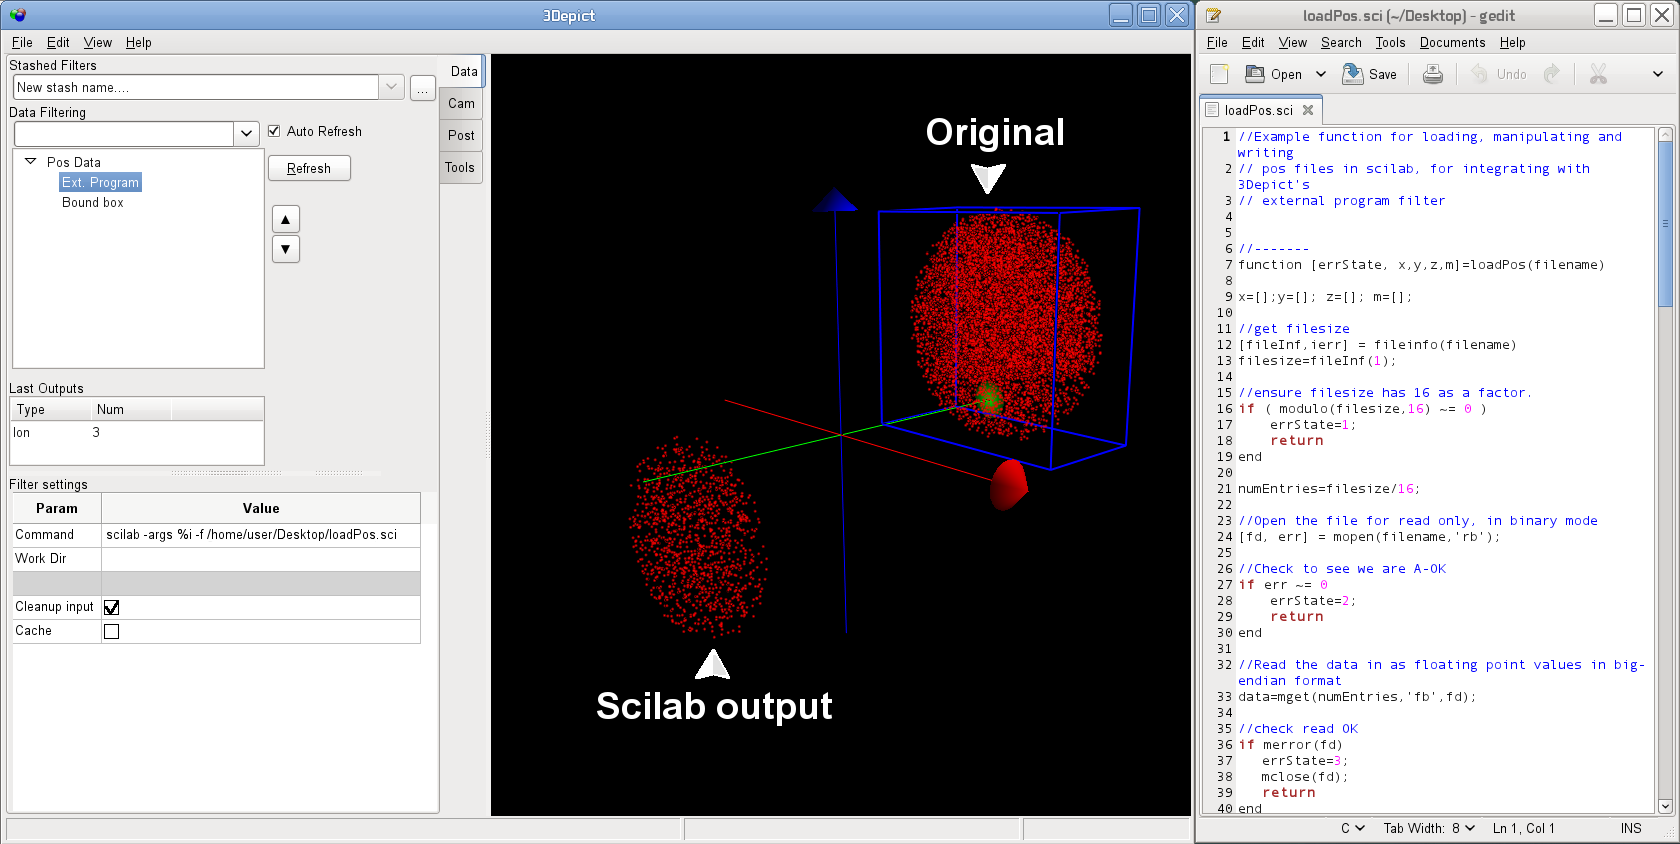
\includegraphics[keepaspectratio=true,width=0.9 \textwidth]{./figures/externalProgScilab.png}
 \caption{Example program screenshot using the \emph{Scilab} sample script. The \%i value in the command line instructs \emph{3Depict} to take the first (and only the first) ion stream, and save it as an input file for the external program. }
 \label{fig:externalProgScilabSample}
 % externalProgBash.png: 1381x875 pixel, 72dpi, 48.71x30.86 cm, bb=0 0 1381 875
\end{center}
\end{figure}

Note that as shown in the figure \emph{Scilab} is called using its `-args' parameter, which avoids \emph{Scilab} from attempting to parse the arguments you wish to pass to the script as its own. Further note that this example will not work if any filename or directory (including the working directory) contains a space, due to this behaviour. In this case, \emph{3Depict} was launched from its own folder, which does not contain a space.

\begin{verbatim}
 //Example function for loading, manipulating and writing 
// pos files in scilab, for integrating with 3Depict's 
// external program filter


//-------
function [errState, x,y,z,m]=loadPos(filename)

x=[];y=[]; z=[]; m=[];

//get filesize
[fileInf,ierr] = fileinfo(filename)
filesize=fileInf(1);

//ensure filesize has 16 as a factor.
if ( modulo(filesize,16) ~= 0 ) 
    errState=1;
    return
end

numEntries=filesize/16;

//Open the file for read only, in binary mode
[fd, err] = mopen(filename,'rb');

//Check to see we are A-OK
if err ~= 0
    errState=2;
    return
end    

//Read the data in as floating point values in big-endian format
data=mget(numEntries,'fb',fd);

//check read OK
if merror(fd)
   errState=3;
   mclose(fd);
   return
end

//Unsplice data, which was stored as xyzmxyzmxyzm...
x=data(1:4:$)';
y=data(2:4:$)';
z=data(3:4:$)';
m=data(4:4:$)';

clear data;

mclose(fd)

errState=0;

endfunction

function err=writePos(filename,x,y,z,m)
    //Check that the array sizes match
    sizes = [ length(x), length(y),length(z),length(m)];
    if max(sizes) ~= min(sizes) 
        err=1;
        return
    end
    
    //Open the file write, in binary mode
    [fd, errState] = mopen(filename,'wb');
    
    if(errState)
        err=2;
        return;
    end
    
    //Build a matrix to dump the data into 
    // in xyzmxyzmxyzm form 
    data=zeros(sizes(1)*4,1);
    data(1:4:$) = x;
    data(2:4:$) = y;
    data(3:4:$) = z;
    data(4:4:$) = m;     
 
    mput(data,'fb',fd);
    
    //Check for io error
    if merror(fd) ~=0
        mclose(fd);
        err=3;
        return;
    end
    
    err=0;
    mclose(fd);
endfunction

//-------

//START OF SCRIPT

//Inform scilab we may need lots of ram.
stacksize('max'); 

//Strip out the script arguments from the general scilab arguments
argsArray=sciargs();
realArgs=[];
numArgs =length(length(argsArray)); //'cause length() is dumb on strings.
for i=1:numArgs
    if argsArray(i) == '-args' & i != length(argsArray);
        realArgs=argsArray(i+1:$);
    end
end

if( length(argsArray) == 0)
    error('no file to open!');
end

//Load the first argument
[errState, x, y, z, m] = loadPos(realArgs(1));
if errState
    error( strcat(['Unable to load posfile, :( ' realArgs(1)]));
else
    printf('Opened file: %s ',realArgs(1));
end


//Draw the point cloud
scf
drawlater
plot3d1(x,y,z)
f=gcf();
pointCloud=f.children.children;
pointCloud.surface_mode="off";
pointCloud.mark_mode="on";
drawnow


//plot a histogram of m, avoiding the error where m has no span
// by artifically adding two elements, if needed.
scf();
if max(m) ~= min(m)
    histplot(100,m);
else
    histplot(100,[min(m)-1; m; max(m)+1]);
    
end


//Now shift each point around 
x=x-1;
y=y-1;
z=z-1;


//now write the file back
err=writePos('output.pos',x,y,z,m);
if  err~= 0
    error('failed to write posfile, :(');
end

//Kill Scilab, because were done and would like to go back to 3Depict.
exit



\end{verbatim}




\subsubsection{Python}
This example demonstrates using \emph{Python} to interact with \emph{3Depict}. The following example does very little - it simply loads all input pos files (due to the \%I in the program invocation), and merges the contents. The results of the computation are shown in Figure~\ref{fig:externalProgPythonSample}.

\begin{figure}
\begin{center}
 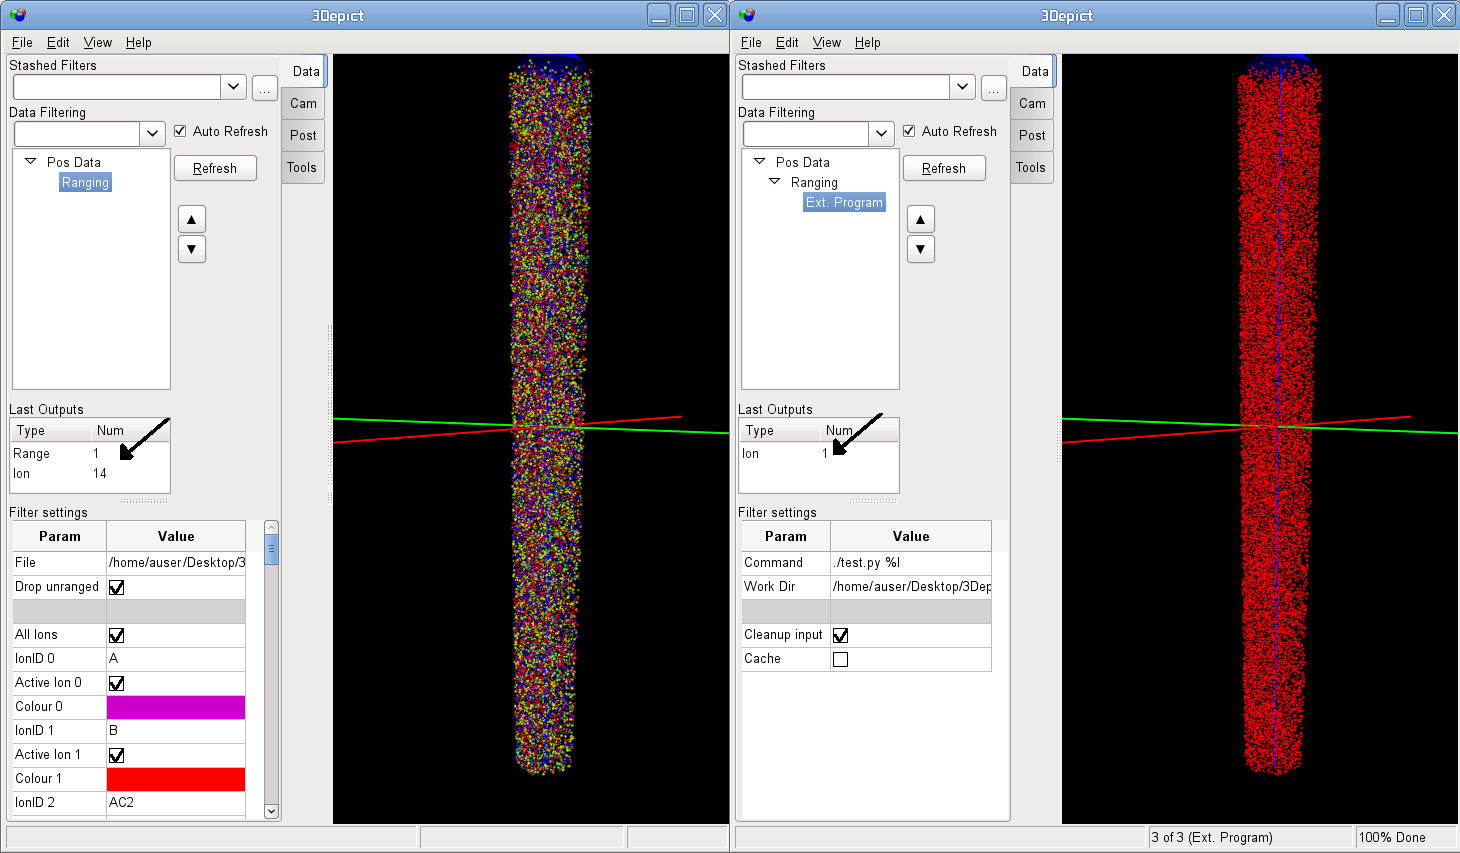
\includegraphics[keepaspectratio=true,width=0.85 \textwidth]{./figures/externalProgPython.png}
 \caption{Example program screenshot without and with the Python test example present. Note that the program merges ion streams into a single pos file, which is re-loaded as a single ion stream, as marked by the arrows.}
 \label{fig:externalProgPythonSample}
 % externalProgBash.png: 1381x875 pixel, 72dpi, 48.71x30.86 cm, bb=0 0 1381 875
\end{center}
\end{figure}

\begin{verbatim}
#!/usr/bin/python

import sys
import os 


#Function to append the contents of one file to another
def appendFile(sourceFile,targetFile):
	try : 
        fileSrc = open(sourceFile,"rb")
        fileTarget = open(targetFile,"ab")
    
        #Extremely inefficient!!
        byte = fileSrc.read(1)
        while byte != "" :
            fileTarget.write(byte)
            byte=fileSrc.read(1)

    except IOError:
        return 1

    return 0

def main():
    argv = sys.argv
    #Name of file that we will dump our results to
    OUTPUT_POSFILE="output.pos"

    #Remove any old files from previous runs
    if os.path.isfile(OUTPUT_POSFILE) :
        os.remove(OUTPUT_POSFILE)


    # do nothing if we have no arguments
    if(len(argv) < 2) :
        return 0;

    #Loop over all our inputs, then for .pos files, 
    # create one big file with all data merged 
    for i in argv[1:] : 
        print "given file :" + i

        fileExt = i[-3:];
        if fileExt  == "pos" :
            if appendFile(i,OUTPUT_POSFILE):
                return 1; #Output to file failed, for some reason
            else : 
                print "appended file to " + OUTPUT_POSFILE

        else :
            #Filename did not end in .pos, lets ignore it.
            print "File :" + i + " does not appear to be a pos file"


    return 0

if __name__ == "__main__":
    sys.exit(main())
\end{verbatim}

\subsubsection{Bash}

The following trivial program shows how \emph{3Depict} can be used send data to and from Bourne Again SHell (\emph{BASH}) programs. \emph{3Depict} was launched with one pos file, and an external program filter, as shown in Figure~\ref{fig:externalProgBashSample}. The script used in the test, named ``test.sh'' and placed in the specified working directory (see figure), is given below. The object of the script is only to demonstrate that the script can be used to perform arbitrary actions, not to perform any actual data manipulations.

\begin{figure}
\begin{center}
 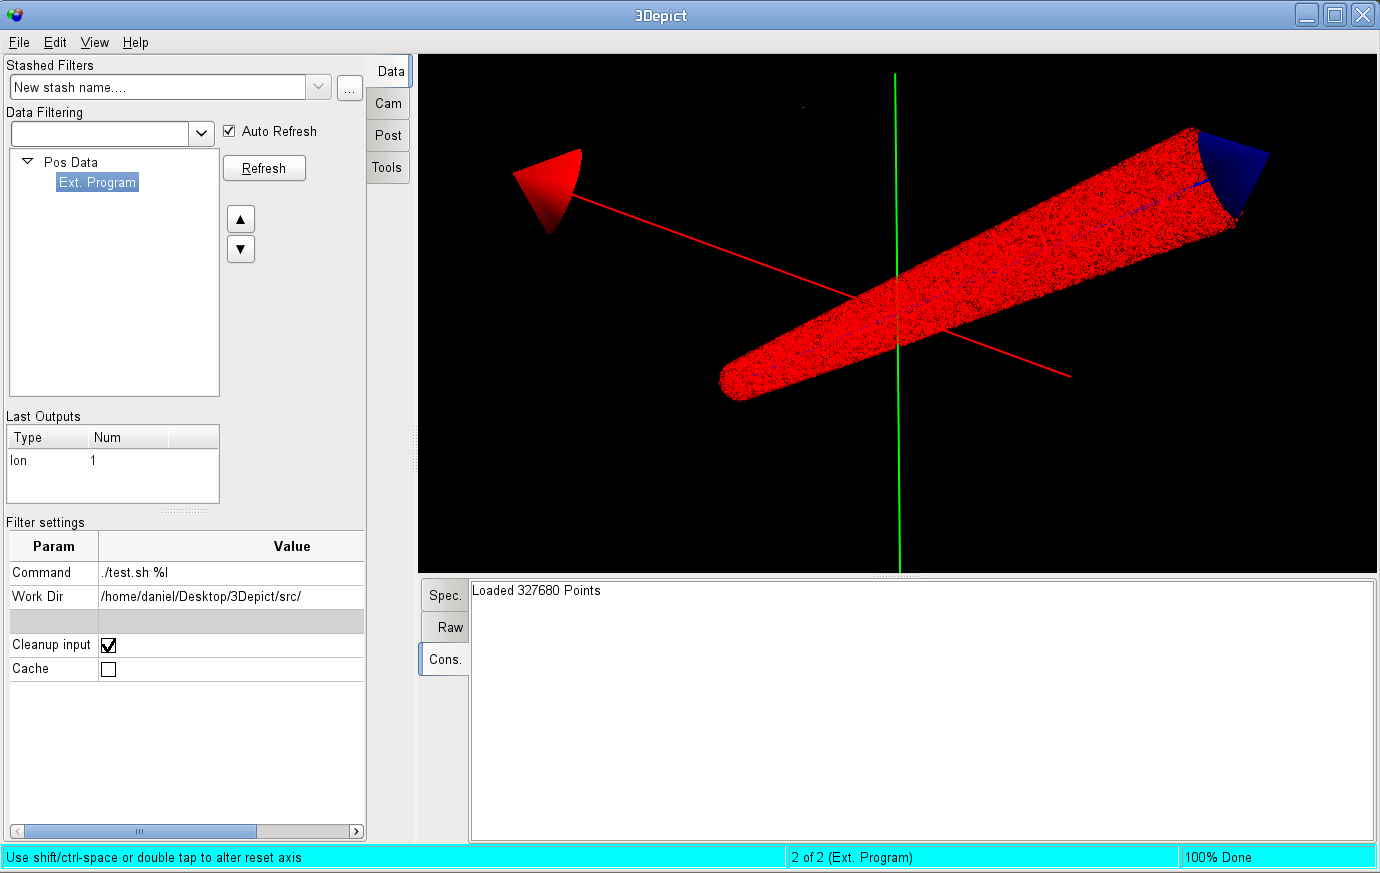
\includegraphics[keepaspectratio=true,width=0.85 \textwidth]{./figures/externalProgBash.png}
 \caption{Example program screenshot when using the BASH test example.}
 \label{fig:externalProgBashSample}
 % externalProgBash.png: 1381x875 pixel, 72dpi, 48.71x30.86 cm, bb=0 0 1381 875
\end{center}
\end{figure}

\begin{verbatim}
#!/bin/bash

BYTES_PER_RECORD=16
echo "Num args : "$#
echo "Working Directory:"  $(pwd)

#Cleanup any previous script-output file
rm script-output-3Depict-input.pos

for (( i=1; i<=$#; i++ )); 
do
        #Get the name of the input file
        eval arg=\$$i
        echo "Input file: $arg"

        #Print some info about the file  
        echo "File size:" $(filesize $arg) " Bytes"
        NUM_IONS=$(expr $(filesize $arg) / $BYTES_PER_RECORD) 
        echo "Num Ions:" $NUM_IONS 

        #Copy the output into the working directory, so that 3Depict's 
        # scanning of the working directory
        # for .pos files will find it
        cat $arg >> script-output-3Depict-input.pos
done 

exit 0
\end{verbatim}

The output from running the refresh cycle is given, as it appears on the program console (to replicate this mac/windows users may need to redirect the output to a file in order to see the output text (this can be done in bash), or mac users may launch \emph{3Depict} from terminal.app).

Firstly, note that the \emph{same file} is written to each time - \emph{3Depict} does not delete the ``script-output-3Depict-input.pos``, so if this is named differently between refreshes, multiple pos files would be generated and \emph{3Depict} would load them all. Finally, the statement \texttt{exit 0} is used to ensure that \emph{3Depict} knows that the program terminated succesfully. Recall that returning a nonzero value will inform \emph{3Depict} that some error occured during processing, and thus it will abort further data processing.

\begin{verbatim}
Working Directory: /home/username/3Depict/src
Input file: /home/username/3Depict/src//inputData/pointdataDNUlfP.pos
File size: 5242880  Bytes
Num Ions: 327680
\end{verbatim}

The output from the program will be similar to the following text.
\begin{verbatim}
given file :/home/auser/Desktop/3Depict/src//inputData/pointdatad7hfUw.pos
appended file to output.pos
\end{verbatim}

\subsubsection{C/C++}
For \emph{C/C++}, an example is given. The example here is somewhat more complex than the rest, as in this case, we do not simply treate the data as a series of bytes, bt we additionally perform the data transformation steps required to get it into a usable form (ie as a list of correctly ordered bytes in memory, in a useful variable). This was not done for the previous examples.

Note that as C/C++ are compiled languages, it is necessary to be able to be able to generate a binary (executable) version of the program - this procedure is not described here, but users are encouraged to be comfortable with this process before attempting to implement the following examples for themselves. The exact procedure for doing this is outside of the scope for this document - you will require a compiler, such as \emph{gcc}'s \emph{g++} compiler, which you will most likely want to install from some form of package management system, such as the \emph{APT}, \emph{yum} or \emph{zypper} systems on linux, \emph{Xcode} or \emph{Macports} on Mac OSX, or \emph{Cygwin} or \emph{tdm-gcc/msys} under windows. Being able to compile a program file to produce an executable binary (under windows `EXE') that consists only of \texttt{int main() \{\} } is a definite prerequisite.

For this program, once your compiler is installed, and assuming you use \emph{gcc}, the normal procedure is to place the following code into a text file called \texttt{example.cpp}, then run \texttt{g++ example.cpp -Wall -o example}, to produce the binary. You must be execute that command in the same folder as the example.cpp file is located. 

This produces a binary file, called ``example'' under linux/OSX or ``example.exe'' under windows, now setting up \emph{3Depict} as per Figure~\ref{fig:externalProgCppSample}, several ranged ionstreams are passed to the program, which are merged into a single file. This single file is detected automatically by \emph{3Depict}, as it is a file ending in ``.pos'', and is located in the working directory - it is thus assumed to be loadable.

\begin{figure}
\begin{center}
 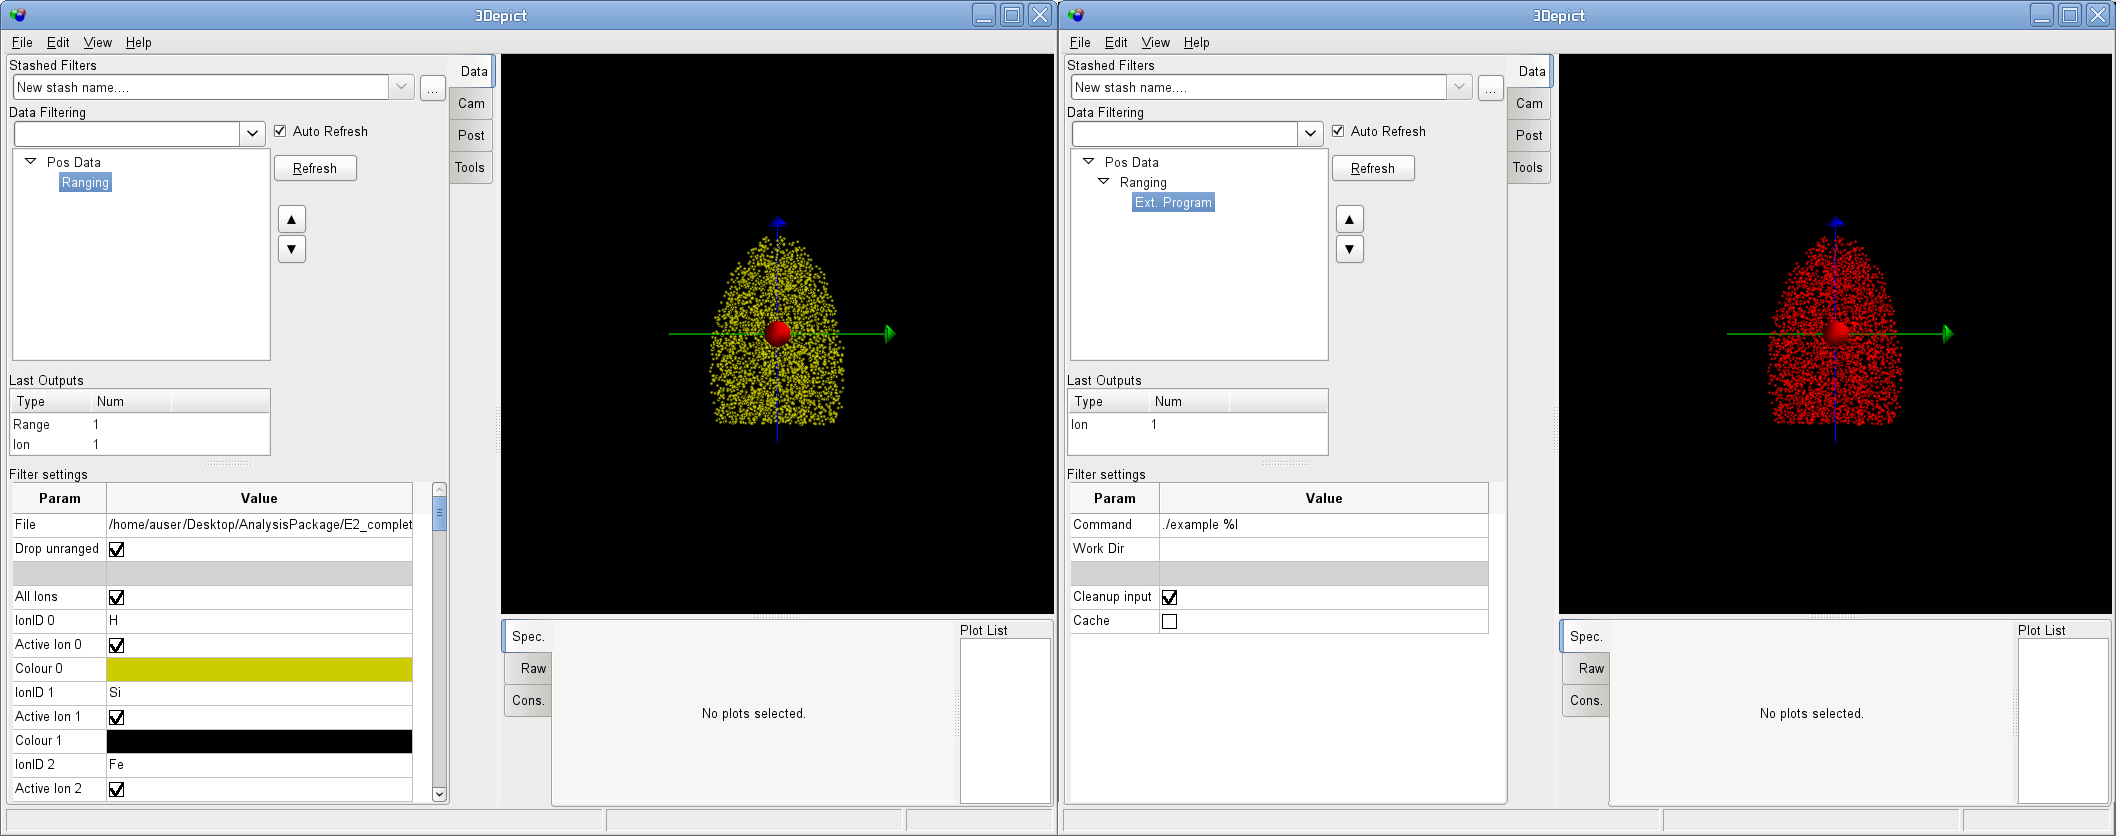
\includegraphics[keepaspectratio=true,width=0.85 \textwidth]{./figures/externalProgCpp.png}
 \caption{Example program screenshot without and with the C++ test example present..}
 \label{fig:externalProgCppSample}
 % externalProgBash.png: 1381x875 pixel, 72dpi, 48.71x30.86 cm, bb=0 0 1381 875
\end{center}
\end{figure}

\begin{verbatim}
 
#include <iostream>
#include <cstdlib>
#include <vector>
#include <fstream>

using namespace std;

enum
{
    ENDIAN_LITTLE,
    ENDIAN_BIG,
    ENDIAN_DUNNO,
};

int endian=ENDIAN_DUNNO;

const int ENDIAN_TEST=1;

//Run-time detection of CPU endian-ness
//---
inline int is_bigendian() { return (*(char*)&ENDIAN_TEST) == 0 ;}
inline int is_littleendian() { return (*(char*)&ENDIAN_TEST) == 1 ;}

void detectEndianNess()
{
    if(is_littleendian())
        endian=ENDIAN_LITTLE;
    else if (is_bigendian())
        endian=ENDIAN_BIG;
    else 
        endian=ENDIAN_DUNNO;
}
//---

struct POS_DATA
{
    float values[4];
};


//A routine for flipping data bytes around between
// big and little endian IEEE754 format
void floatSwapBytes(float *inFloat)
{
    //Use a union to avoid strict-aliasing error
    union FloatSwapUnion{
       float f;
       char c[4];
    } ;
    FloatSwapUnion fa,fb;
    fa.f = *inFloat;

    fb.c[0] = fa.c[3];
    fb.c[1] = fa.c[2];
    fb.c[2] = fa.c[1];
    fb.c[3] = fa.c[0];

    *inFloat=fb.f;
}

//A not-particularly efficient pos-file loader
// returns true on success, false on failure
bool loadPosFile(const std::string &str,vector<POS_DATA> &p)
{
    //open file for "binary" access mode
    ifstream file(str.c_str(),ios::binary);

    //Check file opened OK
    if(!file)
        return false; //open failed


    //Check filesize (in bytes)
    // we do this by jumping to the end,
    // asking the offset, then jumping back to the start
    // as this is very cross-platform (but probably inefficient)
    file.seekg(0,std::ios::end);
    size_t fileSize=file.tellg();
    file.seekg(0,std::ios::beg);

    //Filesize must be 4 4 byte floats
    if(fileSize %16)
        return false;

    //OK, now read the contents    
    size_t numEntries=fileSize/16;
    POS_DATA pd;
    for(size_t ui=0;ui<numEntries;ui++)
    {
        //Read one POS entry (x,y,z,value)
        file.read((char*)pd.values,16);
    
        if(!file.good())
            return false;    

        //Flip the bytes around to match CPU
        // ordering, if needed (eg all x86/x86-64 systems)
        if(endian == ENDIAN_LITTLE)
        {
            for(unsigned int uj=0;uj<3;uj++)
                floatSwapBytes(pd.values+uj);
        }

        p.push_back(pd);
    }

    return true;
}

bool writePosFile(const std::string &filename,const vector<POS_DATA> &p)
{
    //This function assumes floats are 4 bytes
    if(sizeof(float) !=4)
        return false;

    //Open the file for output
    ofstream file(filename.c_str(),ios::binary);
    if(!file)
        return false;

    if(endian == ENDIAN_LITTLE)
    {
        //On little endian machines, loading is a little complicated
        // as we need to convert the pos output back to big-endian mode
        // first
        float values[4];
        for(size_t ui=0;ui<p.size();ui++)
        {
            for(unsigned int uj=0;uj<4;uj++)
            {
                values[uj]=p[ui].values[uj];
                floatSwapBytes(values+uj);
            }
            file.write((const char*)values,4*sizeof(float));
        }
    }
    else
    {
        //On big endian machines, no conversion is neccesary, just write.
        for(size_t ui=0;ui<p.size();ui++)
            file.write((const char*)p[ui].values,4*sizeof(float));
    }

    //Check that nothing went askew whilst writing the file
    if(!file.good())
        return false;
    
    return true;
}

int main(int argc, const char *argv[])
{
    detectEndianNess();
    
    //Get all filenames from input arguments
    vector<string> args;
    for(int ui=1;ui<argc;ui++)
        args.push_back(argv[ui]);

    //accumulate pos data from all input files
    vector<POS_DATA> p;
    try
    {
        for(size_t ui=0;ui<args.size();ui++)
        {
            cerr << "Opening file" << args[ui] << endl;
            if(!loadPosFile(args[ui],p))
                return 1;
        }
    }
    catch(std::bad_alloc)
    {
        cerr <<"Out of memory" << endl;
        return 2;
    }


    //Write it into one file
    cerr << "Writing output file..";
    if(!writePosFile("someFileOrOther.pos",p))
        return 3;

    cerr <<"Done" << endl;

    return 0;
}

\end{verbatim}

\subsection{Modifying the program}

As \emph{3Depict} is an open source program, you are free to modify it, or to extract useful bits subject to the licence agreement (See Section~\ref{sec:licence}). You will need a knowledge of C++ in order to reasonably understand the components of the program itself. A knowledge of OpenGL and wxWidgets is desirable, but you could pick this up as you went along, and don't really need it for many parts of the program.

This section of the manual is the hardest to write, and the most likely to not be applicable to your context, as it depends heavily on the computer system you are trying to use. Nevertheless, this section will attempt to explain how to get yourself set up to build. To modify the program, you must first be able to build the base version of the program from source code. This is by far easiest under a Linux system, as packaging programs can allow you to auto-import all the needed components to build the program.

\subsubsection{Development tools}
The program was primarily developed using C++ (gcc), and utilises autotools for the build scripts. Some custom Bourne-again shell (BASH) scripts are used to do side tasks, such as dependency retrieval and compilation and .app package building (for OSX, really). Mercurial is used for version control. The program is developed using a private repository, which is synced up to the Sourceforge repository periodically. My personal tools for development are the VIM editor and the command line.  This was primarily developed under a Debian squeeze (testing) system (EEE 901), with some development under OpenSuse. The authors actively maintain the programs' package for Debian, and this is periodically synchronised to Ubuntu's package database. The program is also available under the Fedora platform.
 
The main libraries used for the program are:

\begin{itemize}
\item wxWidgets - User interface, \url{http://www.wxwidgets.org}
\item mathgl - Plot generation, \url{http://www.mathgl.sourceforge.net}
\item ftgl -  3D text, \url{http://www.ftgl.sourceforge.net}
\item libxml2 -  XML parsing and validation, \url{http://xmlsoft.org}
\item qhull -  Convex hull compuations, \url{http://www.qhull.org}
\item gettext and iconv- Internationalisation \url{http://www.gnu.org/software/gettext/}
\item libpng - PNG image reader/writer library \url{http://libpng.org}
\item freetype2 - font loader library \url{http://freetype.org/}
\end{itemize}


\subsubsection{Getting yourself set up}
Compilation instructions vary from operating system to operating system. In increasing order of complexity to generate a compilation, Linux, mac, and windows versions can be built from source. Instructions for compilation change frequently, and the most up to date version is available on the project website.

If you are running a Debian or Debian derived distribution, all you need to do is to run these commands as an admin user \texttt{sudo aptitude install build-essential}, which will install a compiler and the needed build scripts. Then run \texttt{sudo apt-get build-dep 3depict}, this will install all the needed components to install the program.

Once this is done, you can download the latest source code from the website, unzip it, and then run \texttt{./configure \&\& make}. This builds the program. You can now modify any of the files, then recompile it simply running \texttt{make}. By examining the options listed by \texttt{./configure --help}, the configuration of the program can be altered to some extent (\emph{e.g.}, enable/disable debug checks, or computational parallelism).

\subsubsection{Changing stuff}
As \emph{3Depict} is open source, it can be modified in the case any error fixes, extentions or other alterations to the program are  desired. However, a certain level of prerequisite knowledge is necessary to effectively alter the program. If altering code in \emph{3Depict}, You should be familiar with C++, as well as compiling multi-file programs. Depending upon the modification, you may need to have some familiarity with the mathematical problems you need to solve and with libraries used by \emph{3Depict}, such as OpenGL or wxWidgets. 

The internal structure of the program can be more easily seen from the Doxygen documentation, which is listed online, or can be generated from the source files themselves via the Doxygen tool. If you want to have a play around with the code, try getting it to compile first, before trying to change anything. Feel free to drop us a line on the website to ask about the change you want to make, and how it could be most easily achieved in the code.

All you have to do now is to modify the .cpp and .h files to do what you want, this is going to be specific to what you want to do, and thus it is impossible for a ``walkthrough'' to be reasonably written. This is only here as a guide. To get started, the easiest components to change are probably the filters. These have been written to be as independent of the user interface as possible, so you need to know very little (almost nothing) about OpenGL or wxWidgets to modify them. 

Each filter is an object derived from a base class, \texttt{Filter}.  To implement a new filter, you have to derive a new class, eg \texttt{MyFilter}, and implement the pure virtual functions to do what you want. To make it accessible from the user interface, you have to add a new entry in  \texttt{comboFilters\_choices} in the function \texttt{MainWindowFrame::MainWindowFrame($\ldots$)}, in \texttt{MainWindowFrame::OnComboFilter($\ldots$)} in \texttt{3Depict.cpp} as well as in \texttt{makeFilter(\ldots)}. You can probably just copy the relevant bits from a neighbouring filter.

The main purpose of the filter design is is that each filter takes in something, and spits out something - by simply implementing a new filter, a new effect can be achieved. The filter's job is to convert input FilterStreamData, into some other output.  Each filter does all of its work in the \texttt{::refresh} functions. The easiest examples of this will probably be the ion info and transform filters. They might look a bit daunting, but much of the code is simply there to keep things running as fast as it can, and to provide many options. Each filter can only work with its own properties, and that of the FilterStreamData pointers passed into the refresh function. It can really do anything it wants here. The refresh logic will examine the filter outputs to determine their consistency  (both internally, and against the filter data output matrix) when compiled in debugging mode, generating errors on any detected inconsistencies in the output.

To have properties appear up in the left hand panel, you have to implement the \texttt{getProperties($\ldots$)} function -- try copying one that seems closest to your situation. To have these properties take effect, you need to implement the \texttt{setProperties($\ldots$)} function. If you wish to ``peek-ahead'' at the filters coming into the filter (this is a little advanced, but can sometimes be necessary), you have to implement the \texttt{initFilter($\ldots$)} function.

\bibliographystyle{unsrt}
\bibliography{manual}

\end{document}
